\subsection{27 августа. Пер. Перемётный (1А)}
\textit{Метеоусловия: утром, днём, вечером ясно, тепло.}
\begin{figure}[h!]
	\centering
	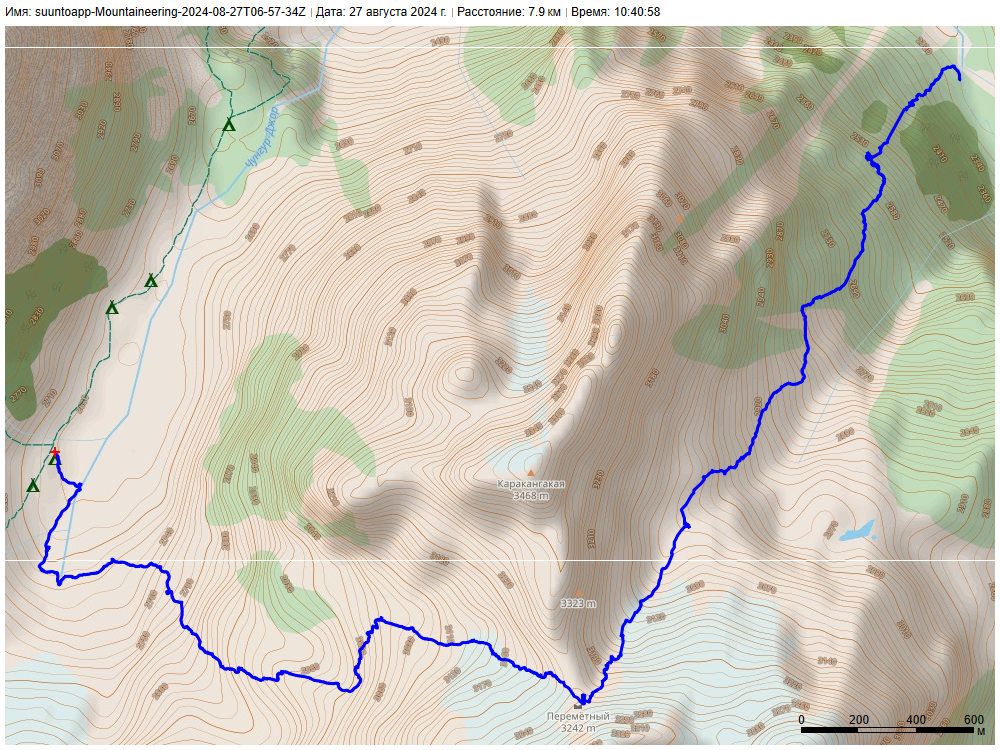
\includegraphics[angle=0, width=0.7\linewidth]{../pics/mini_maps/27}
	\label{fig:mini_27}
\end{figure}

Утром проснулись в 7:00. Погода стояла прекрасная: небо ясное, долину постепенно заливало солнцем. Долго стирались, чинились и сушились, руковод курил какао и размышлял... Перемётный было решено брать!
В 10:00 выдвинулись в сторону перевала. 

\subparagraph{Примечание от руководителя:} ситуация с Перемётным до последнего момента оставалась крайне спорной. С одной стороны, группа, очевидно, не до конца восстановилась после вчерашней непогоды, да и на десятый день похода, который, по опыту, всегда бывает кризисным, уже должна была проявить себя накопленная усталость. С другой стороны, группа, во-первых, не выказывала признаков именно что морального истощения, а во-вторых, была уверенность, что, элементарно, солнце, которое скоро должно было дойти до лагеря, качественно улучшит состояние участников, и под солнцем группа сможет восстановиться даже на ходу. Предполагая, однако, что первый комплекс аргументов всё-таки перевешивает, и сильно колеблясь, руководитель вначале объявил группе об отказе от Перемётного. Однако, оценив реакцию участников, и не услышав явного вздоха облегчения, решил всё же пойти на риск, изменил своё решение, и отдал команду готовиться к выходу на Перемётный.

\begin{figure}[h!]
	\centering
	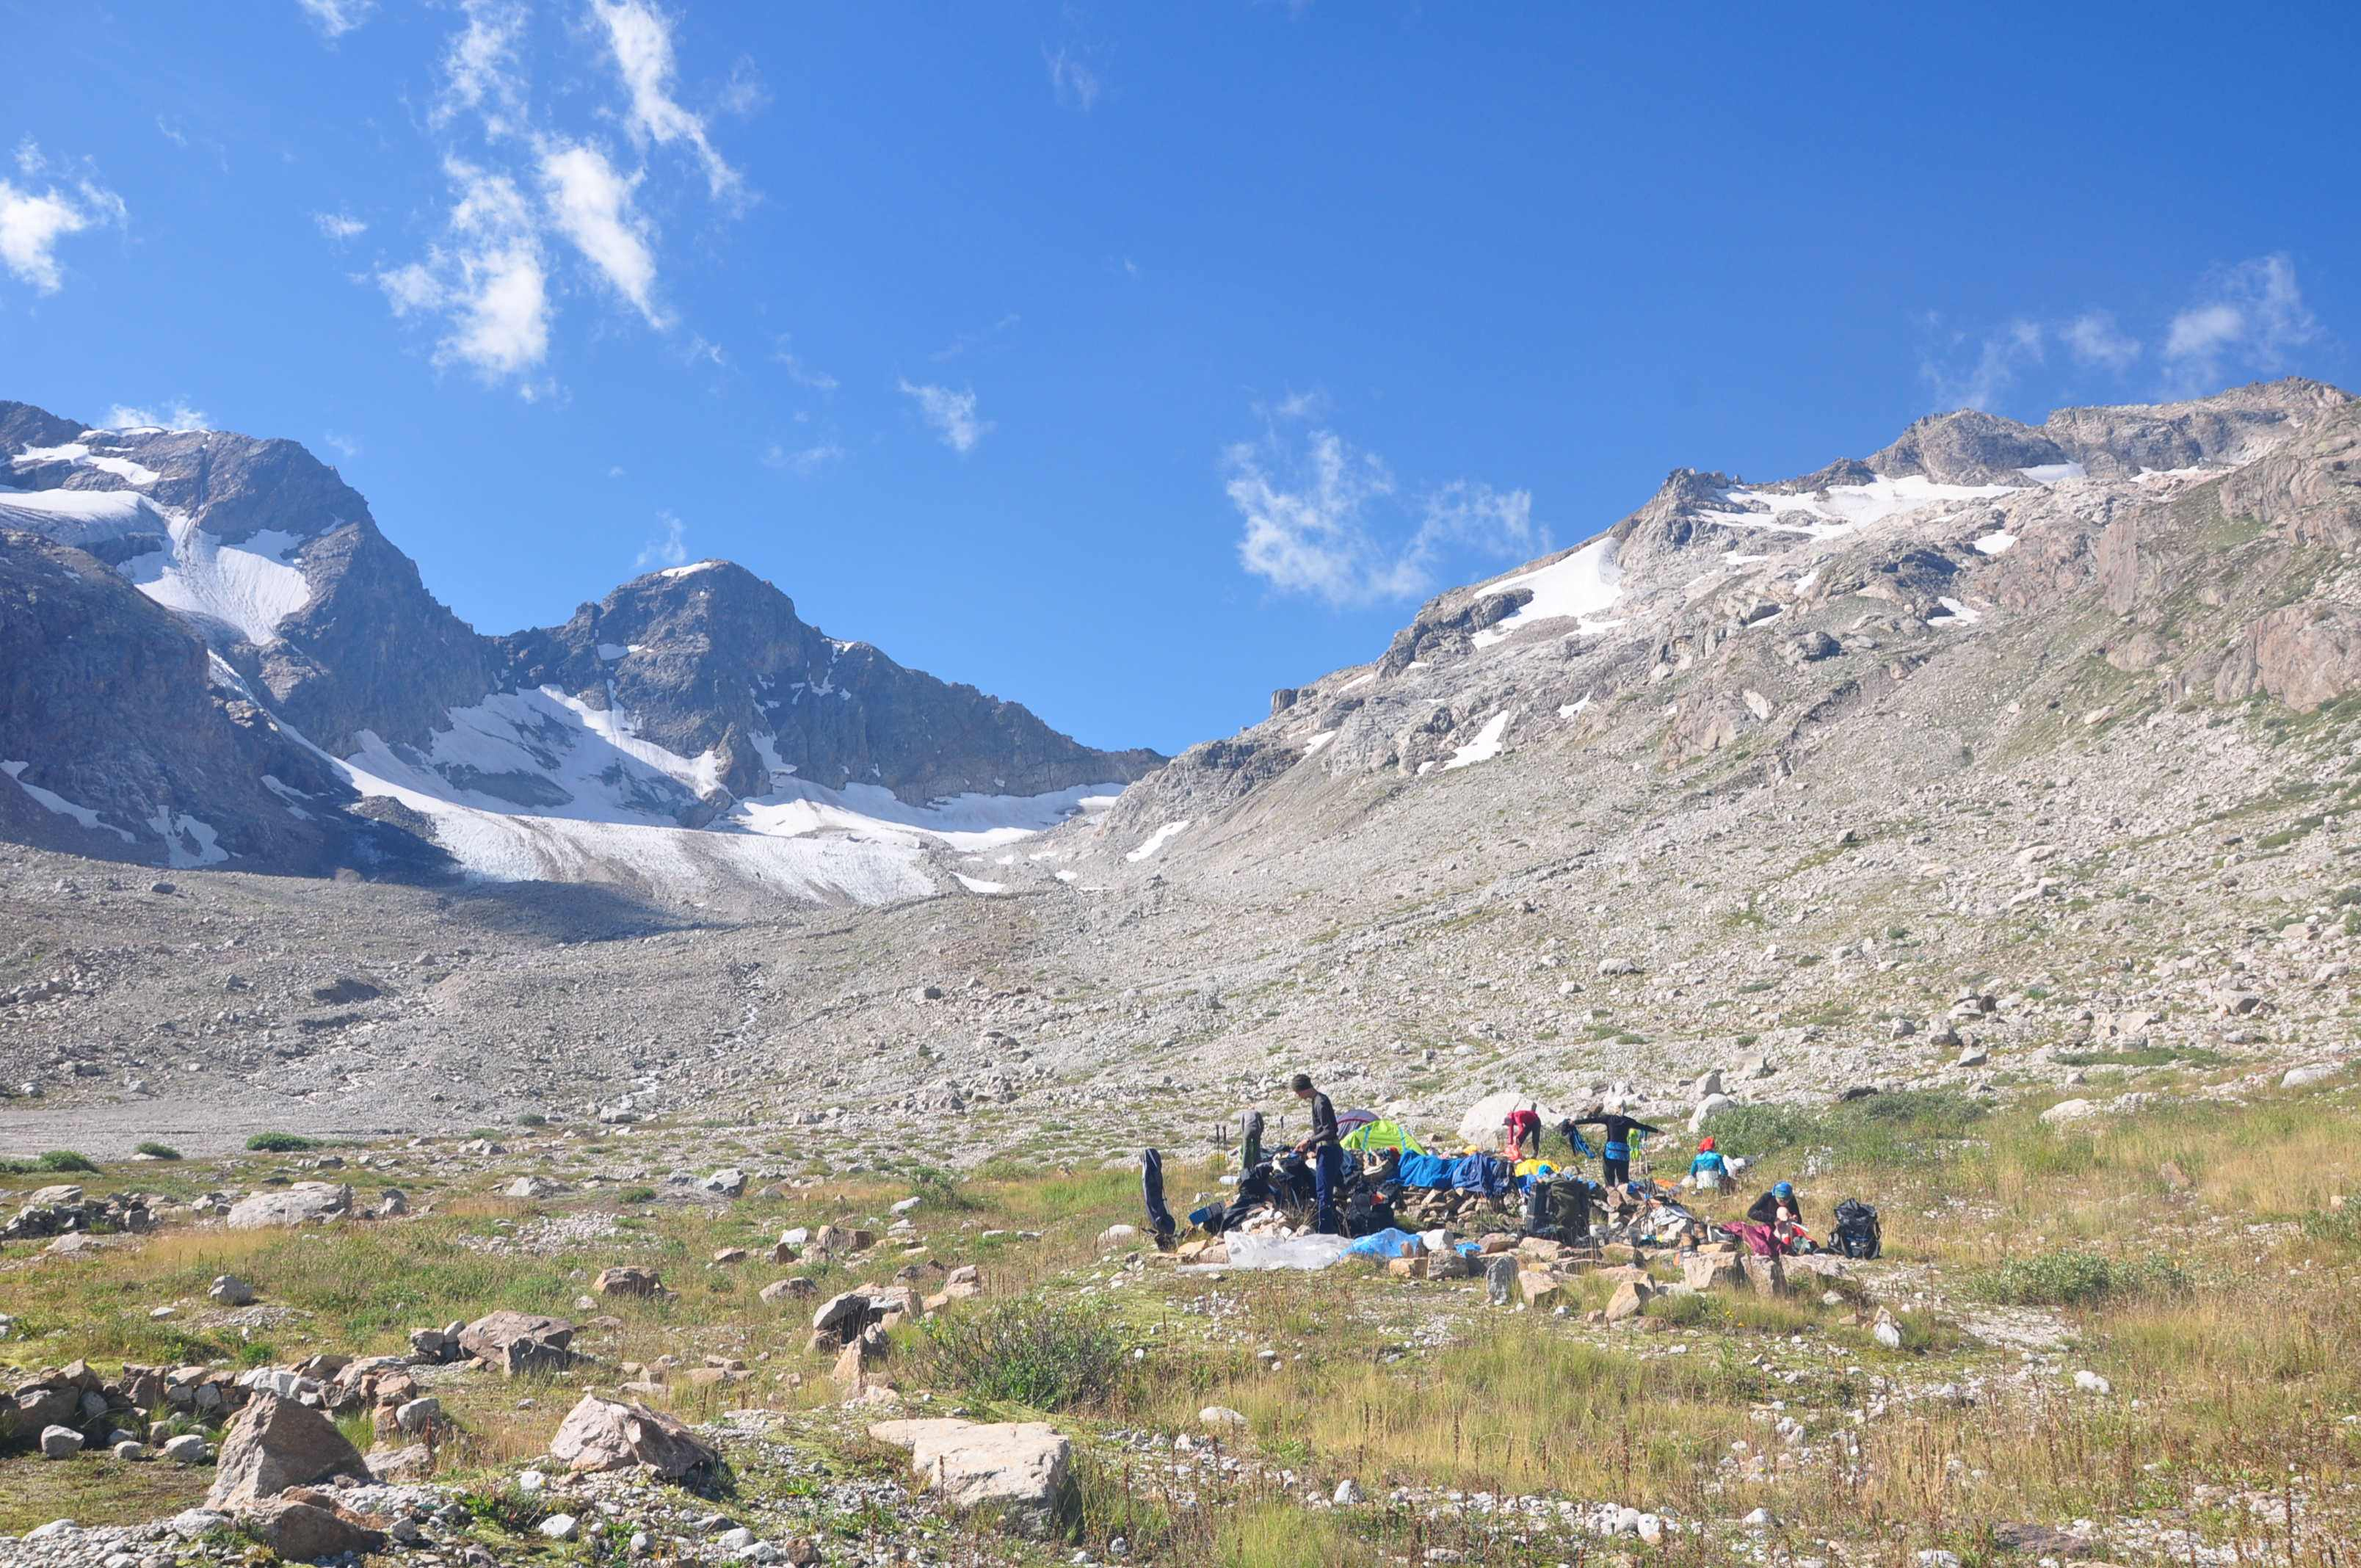
\includegraphics[width=0.7\linewidth]{../pics/DSC_0251.jpg}
	\caption{Утренний лагерь. Активно сушимся.}
	\label{fig:DSC_0251}
\end{figure}

\textbf{Задачей номер раз} было перейти многорукавье реки Чунгур-Джар. По результатам вчерашней разведки была возможность перебродить реку на урочище Аэродром --- при этом некоторые участники могли бы пересечь реку, не замочив ног. Но в ходе дискуссии между руководителем и заместителем было принято решение переходить многорукавье реки в верховьях, поднимаясь так, чтобы рукава было можно было перейти посуху всем. Это оказалось сложнее, чем казалось. Часть группы всё-таки промочила ботинки и усердно их сушила на каждом привале. 

\subparagraph{Примечание от лица руководителя:} Обход р. Чунгур-Джара по верховьям, по моему глубокому убеждению, не стоит затрачиваемых на это усилий. Лично я однозначно рекомендую переходить Чунгур-Джар в районе разлива, напротив стоянок. Лёша планировал перейти реку ещё выше, чем это получилось по факту, но я вынудила группу начать бродить там, чтобы сэкономить время на подъёме по моренным валам. Это решение нами обоими было оценено как неоптимальное. 
\begin{figure}[h!]
	\centering
	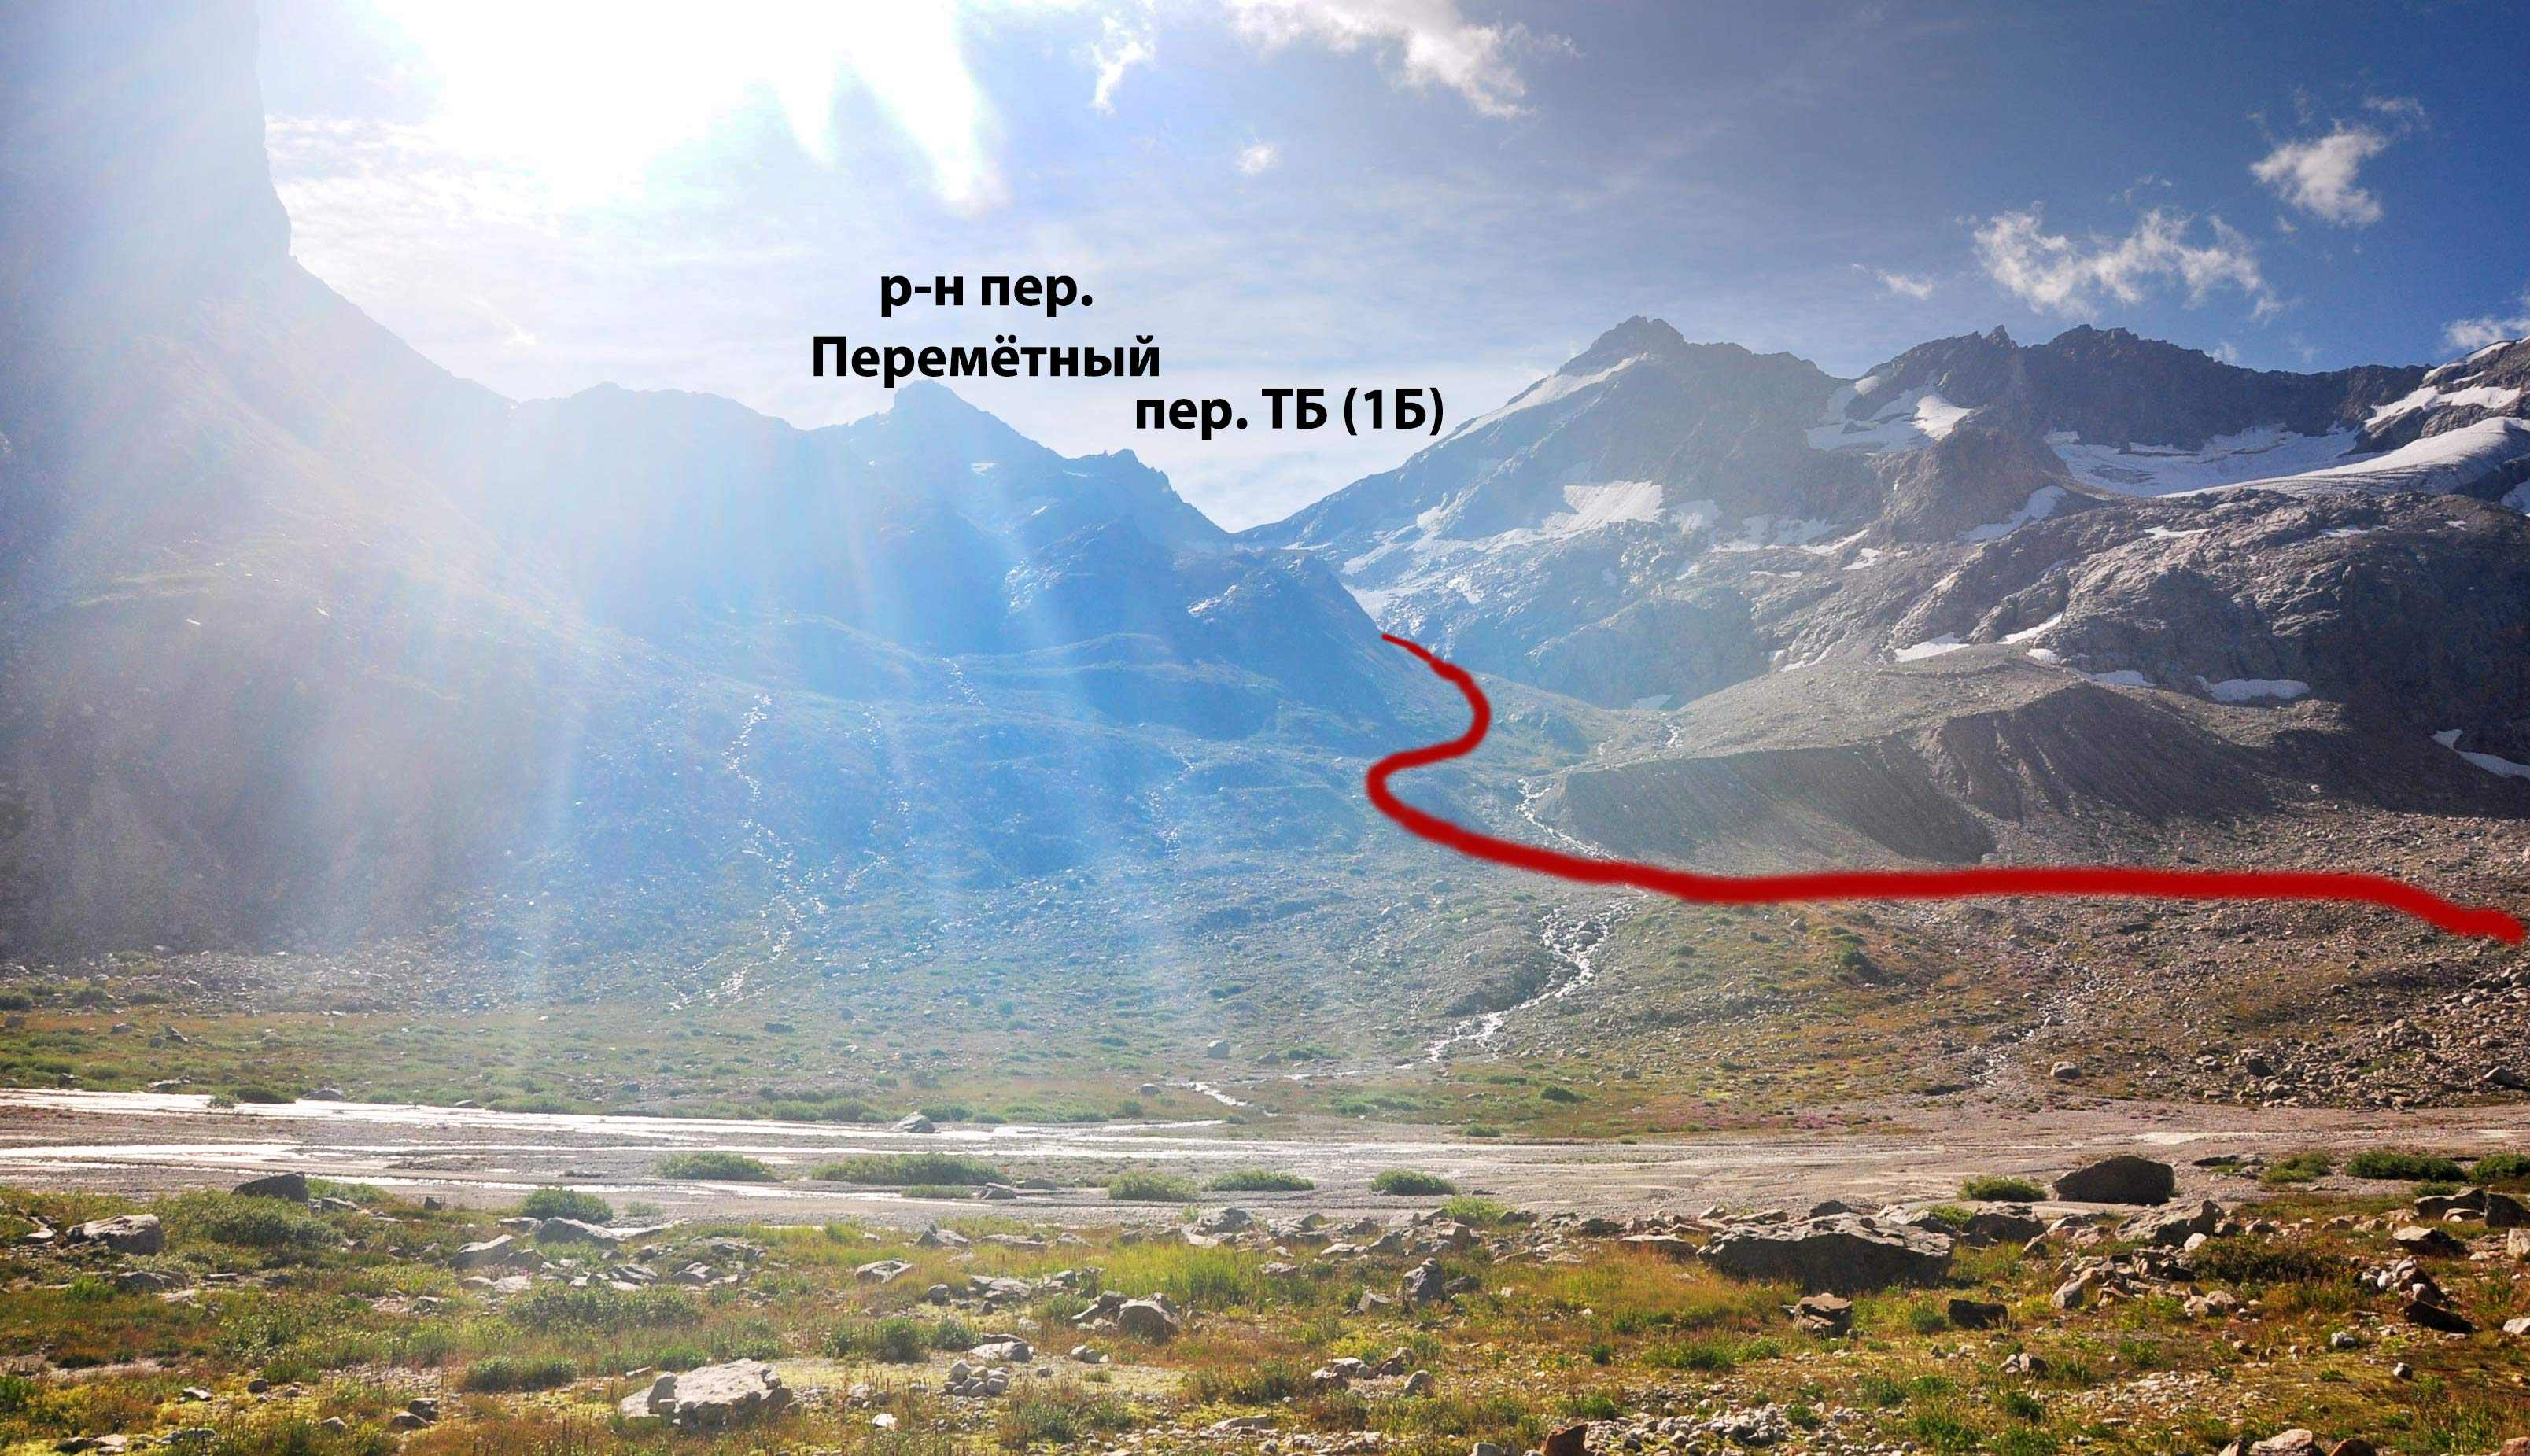
\includegraphics[width=0.7\linewidth]{../pics/DSC_0254.jpg}
	\caption{р. Чунгур-Джар. Нам предстоит перебраться через множество ручейков}
	\label{fig:DSC_0254}
\end{figure}

\begin{figure}[h!]
	\centering
	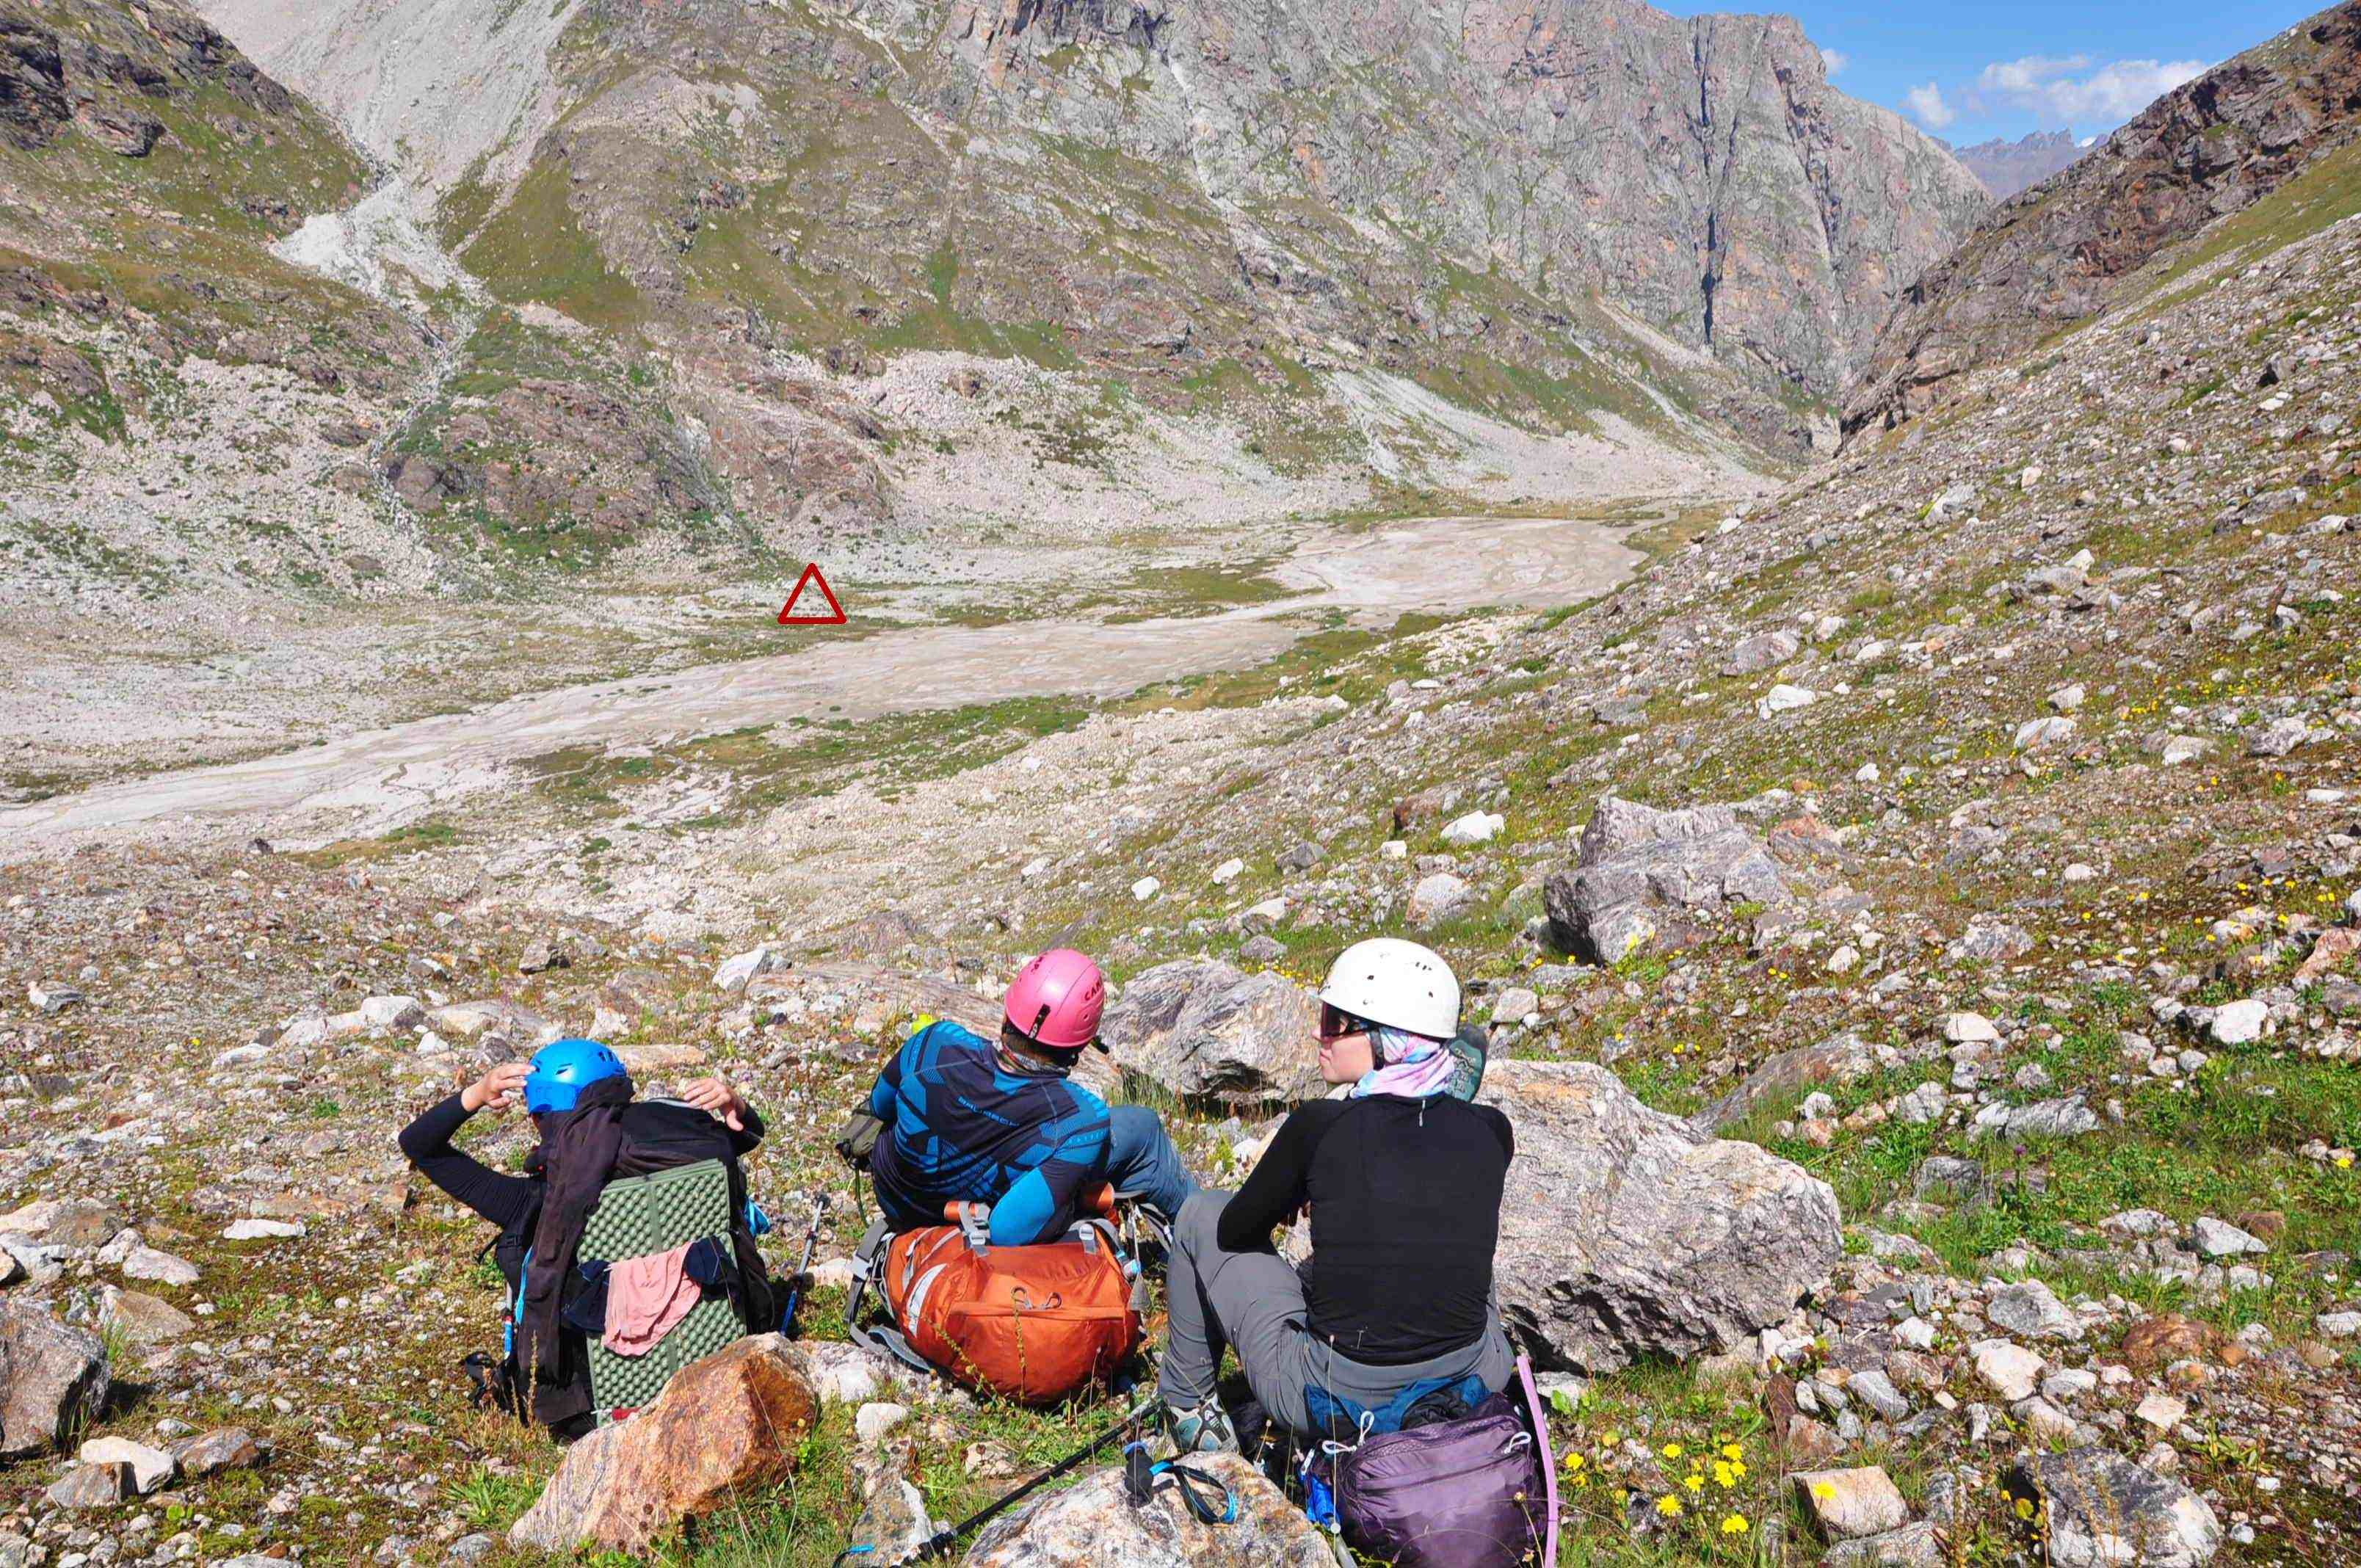
\includegraphics[width=0.7\linewidth]{../pics/DSC_0277.jpg}
	\caption{р. Чунгур-Джар. Перебрались}
	\label{fig:DSC_0277}
\end{figure}

\textbf{Задачей номер два было} пройти подъём на перевал. Поднялись на первую ступень морены по травянисто-осыпному склону, забирая вправо пхд. Далее огибали косым траверсом травянистый «пупырь». В какой-то момент решили подниматься на него практически в лоб --- это оказалось ошибкой: <<пупырь>> оказывается склоном моренного вала, который опоясывает ступень висячей долины с южной стороны. На востоке же начинается другая морена, по которой, собственно, и проходит путь подъёма на Перемётный. Между восточной мореной и южным моренным валом есть понижение, через которое можно пройти, если траверсировать <<пупырь>> --- т.~е. моренный вал с его внешней стороны практически без набора высоты. Нам же пришлось сначала идти по гребню, а затем спускаться по внутренней, осыпной стороне вала, до упомянутого выше понижения, совершая таким образом паразитный сброс. На высоте 2958~м (N43.24135\degree, E42.24827\degree) в 12:33  начали траверс по сыпухе и под небольшой скалой на восточную морену (рис.~\ref{fig:perem_1},\ref{fig:DSC_0280}).

\begin{figure}[h!]
	\centering
	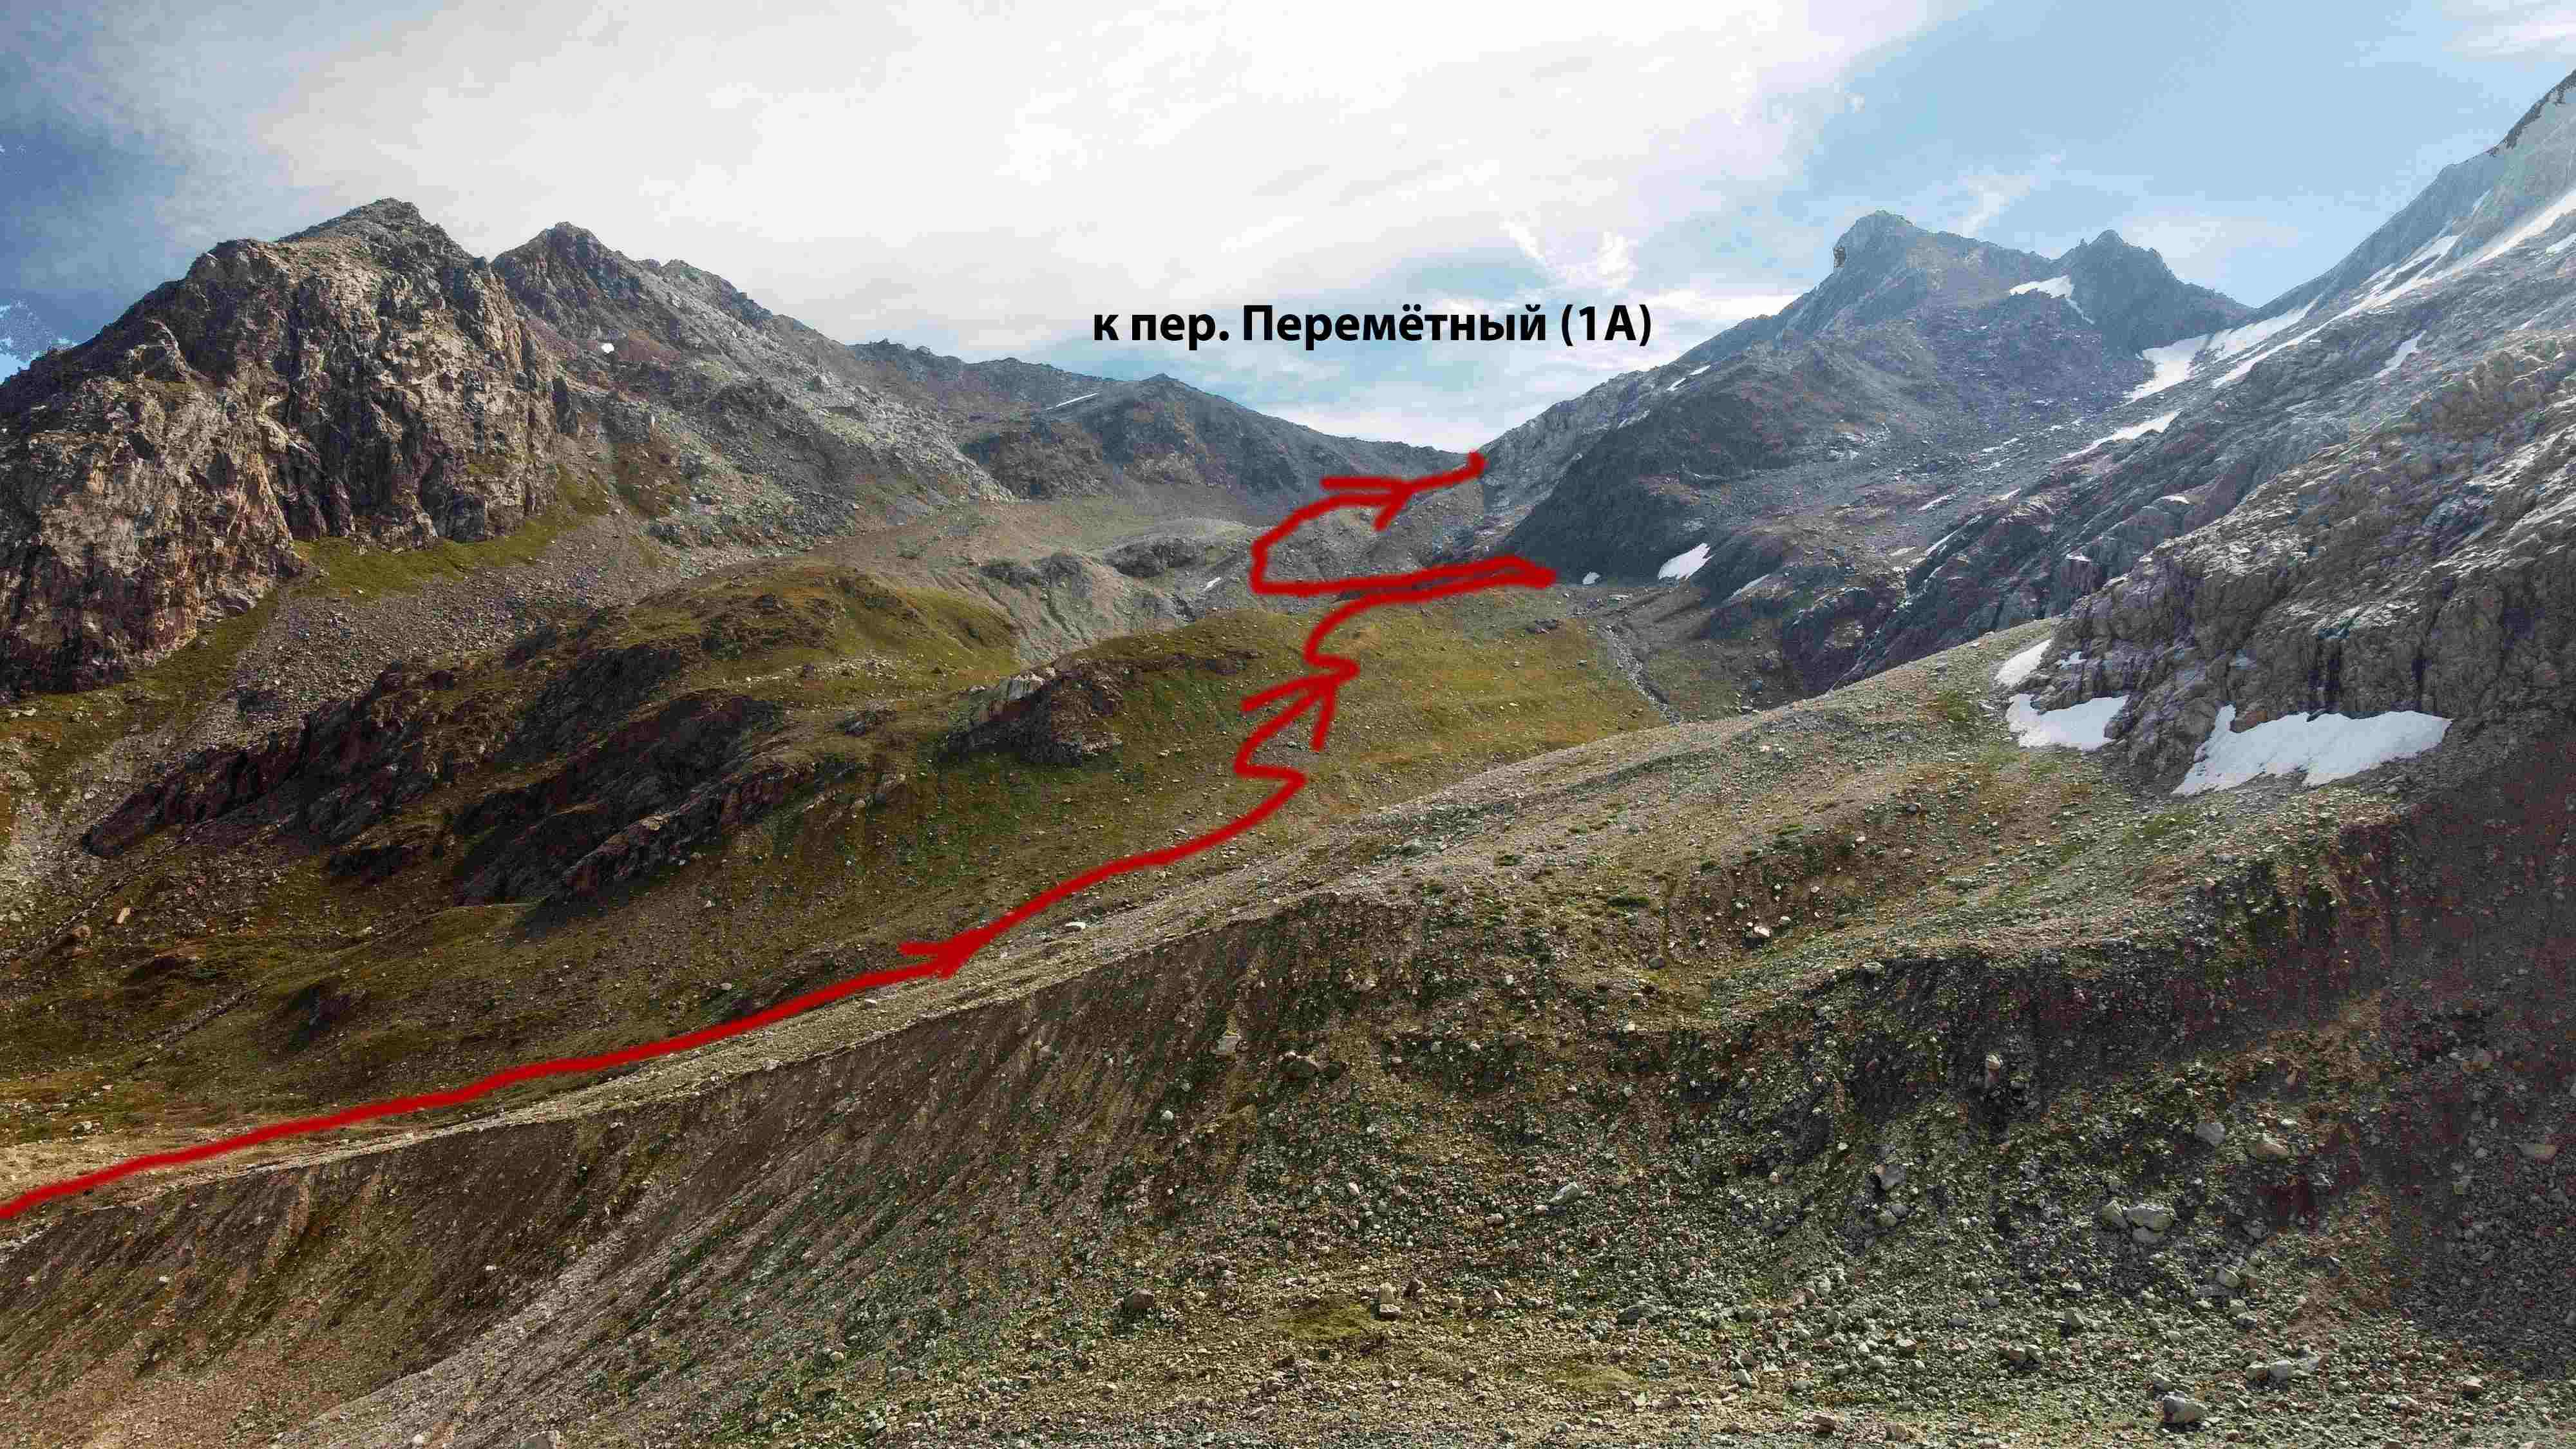
\includegraphics[width=0.7\linewidth]{../pics/perem_1}
	\caption{Начало подъёма к пер. Перемётный из д.р. Чунгур-Джар}
	\label{fig:perem_1}
\end{figure}  

\subparagraph{Примечание от руководителя:} во время траверса восточной морены в направлении с юга на север имеет смысл ориентироваться на большой камень, лежащий на северной стороне склона. Съезжая по осыпи, этот камень образовал небольшой осыпной кулуар --- соответственно, мы обходили этот кулуар справа пхд, выходя затем по гребню на очередную моренную ступень (рис. \ref{fig:DSC_0280}).

\begin{figure}[h!]
	\centering
	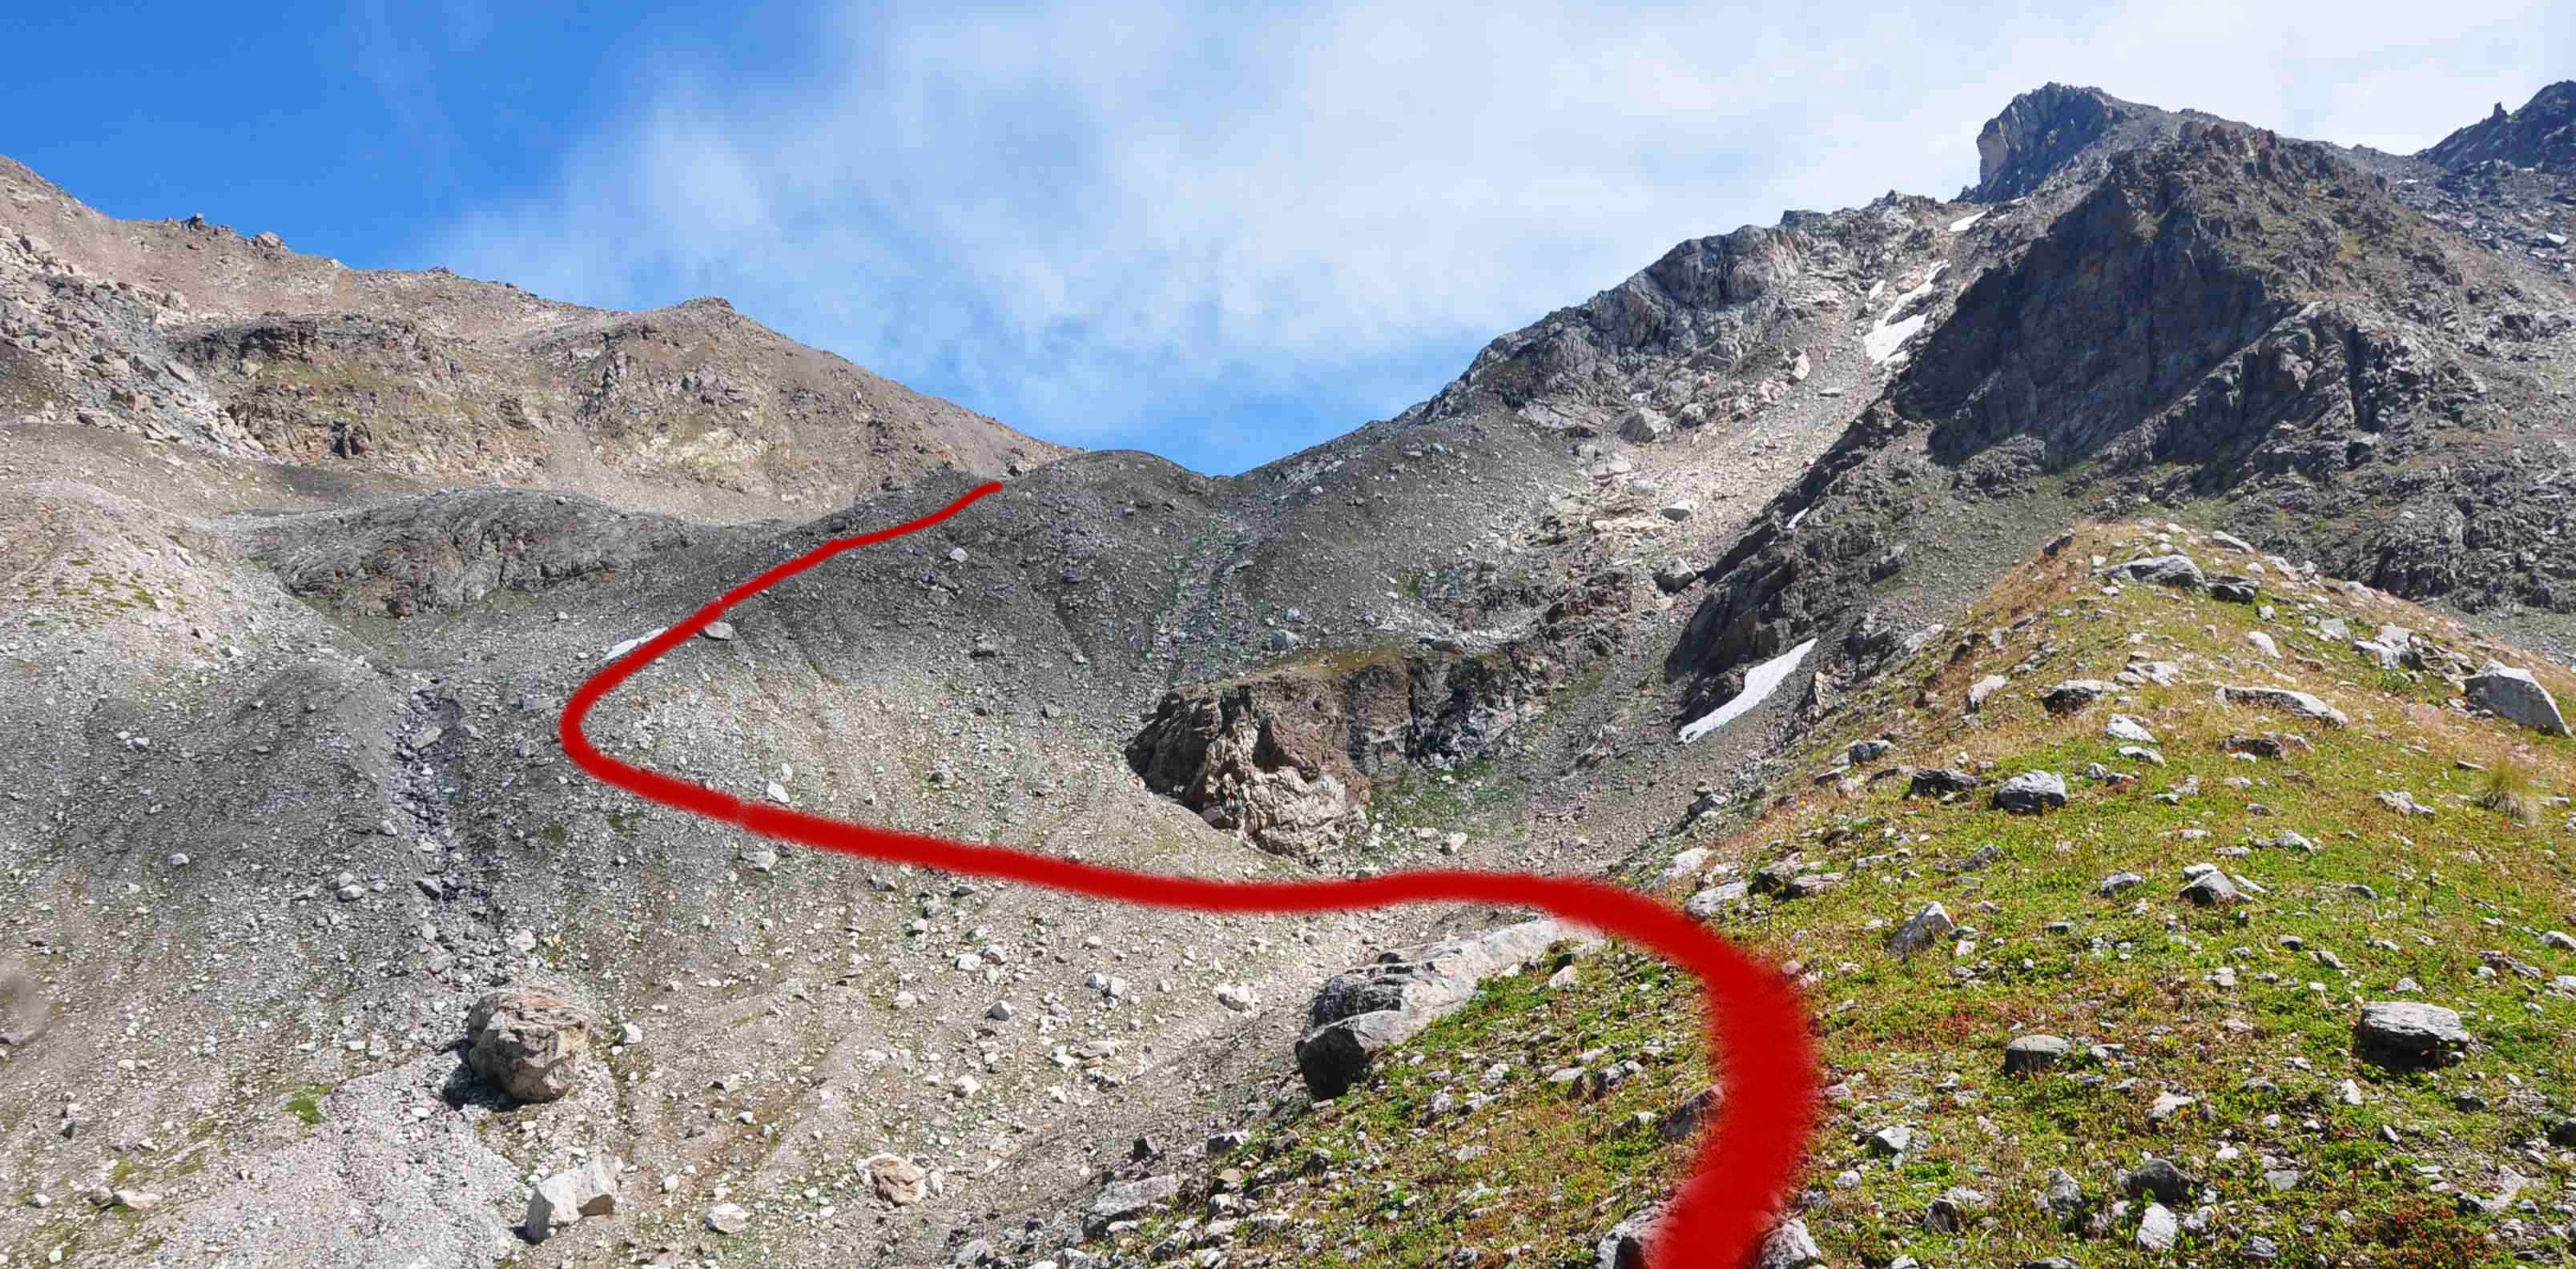
\includegraphics[width=0.7\linewidth]{../pics/DSC_0280.jpg}
	\caption{Траверс по моренам и выход на моренный гребень}
	\label{fig:DSC_0280}
\end{figure}

После этого~--- прямым курсом на перевал. Финальный участок подъёма идёт по пологой средней осыпи и не является трудным ни физически, ни технически, ни психологически (рис.~\ref{fig:DSC_0341}).

\begin{figure}[h!]
	\centering
	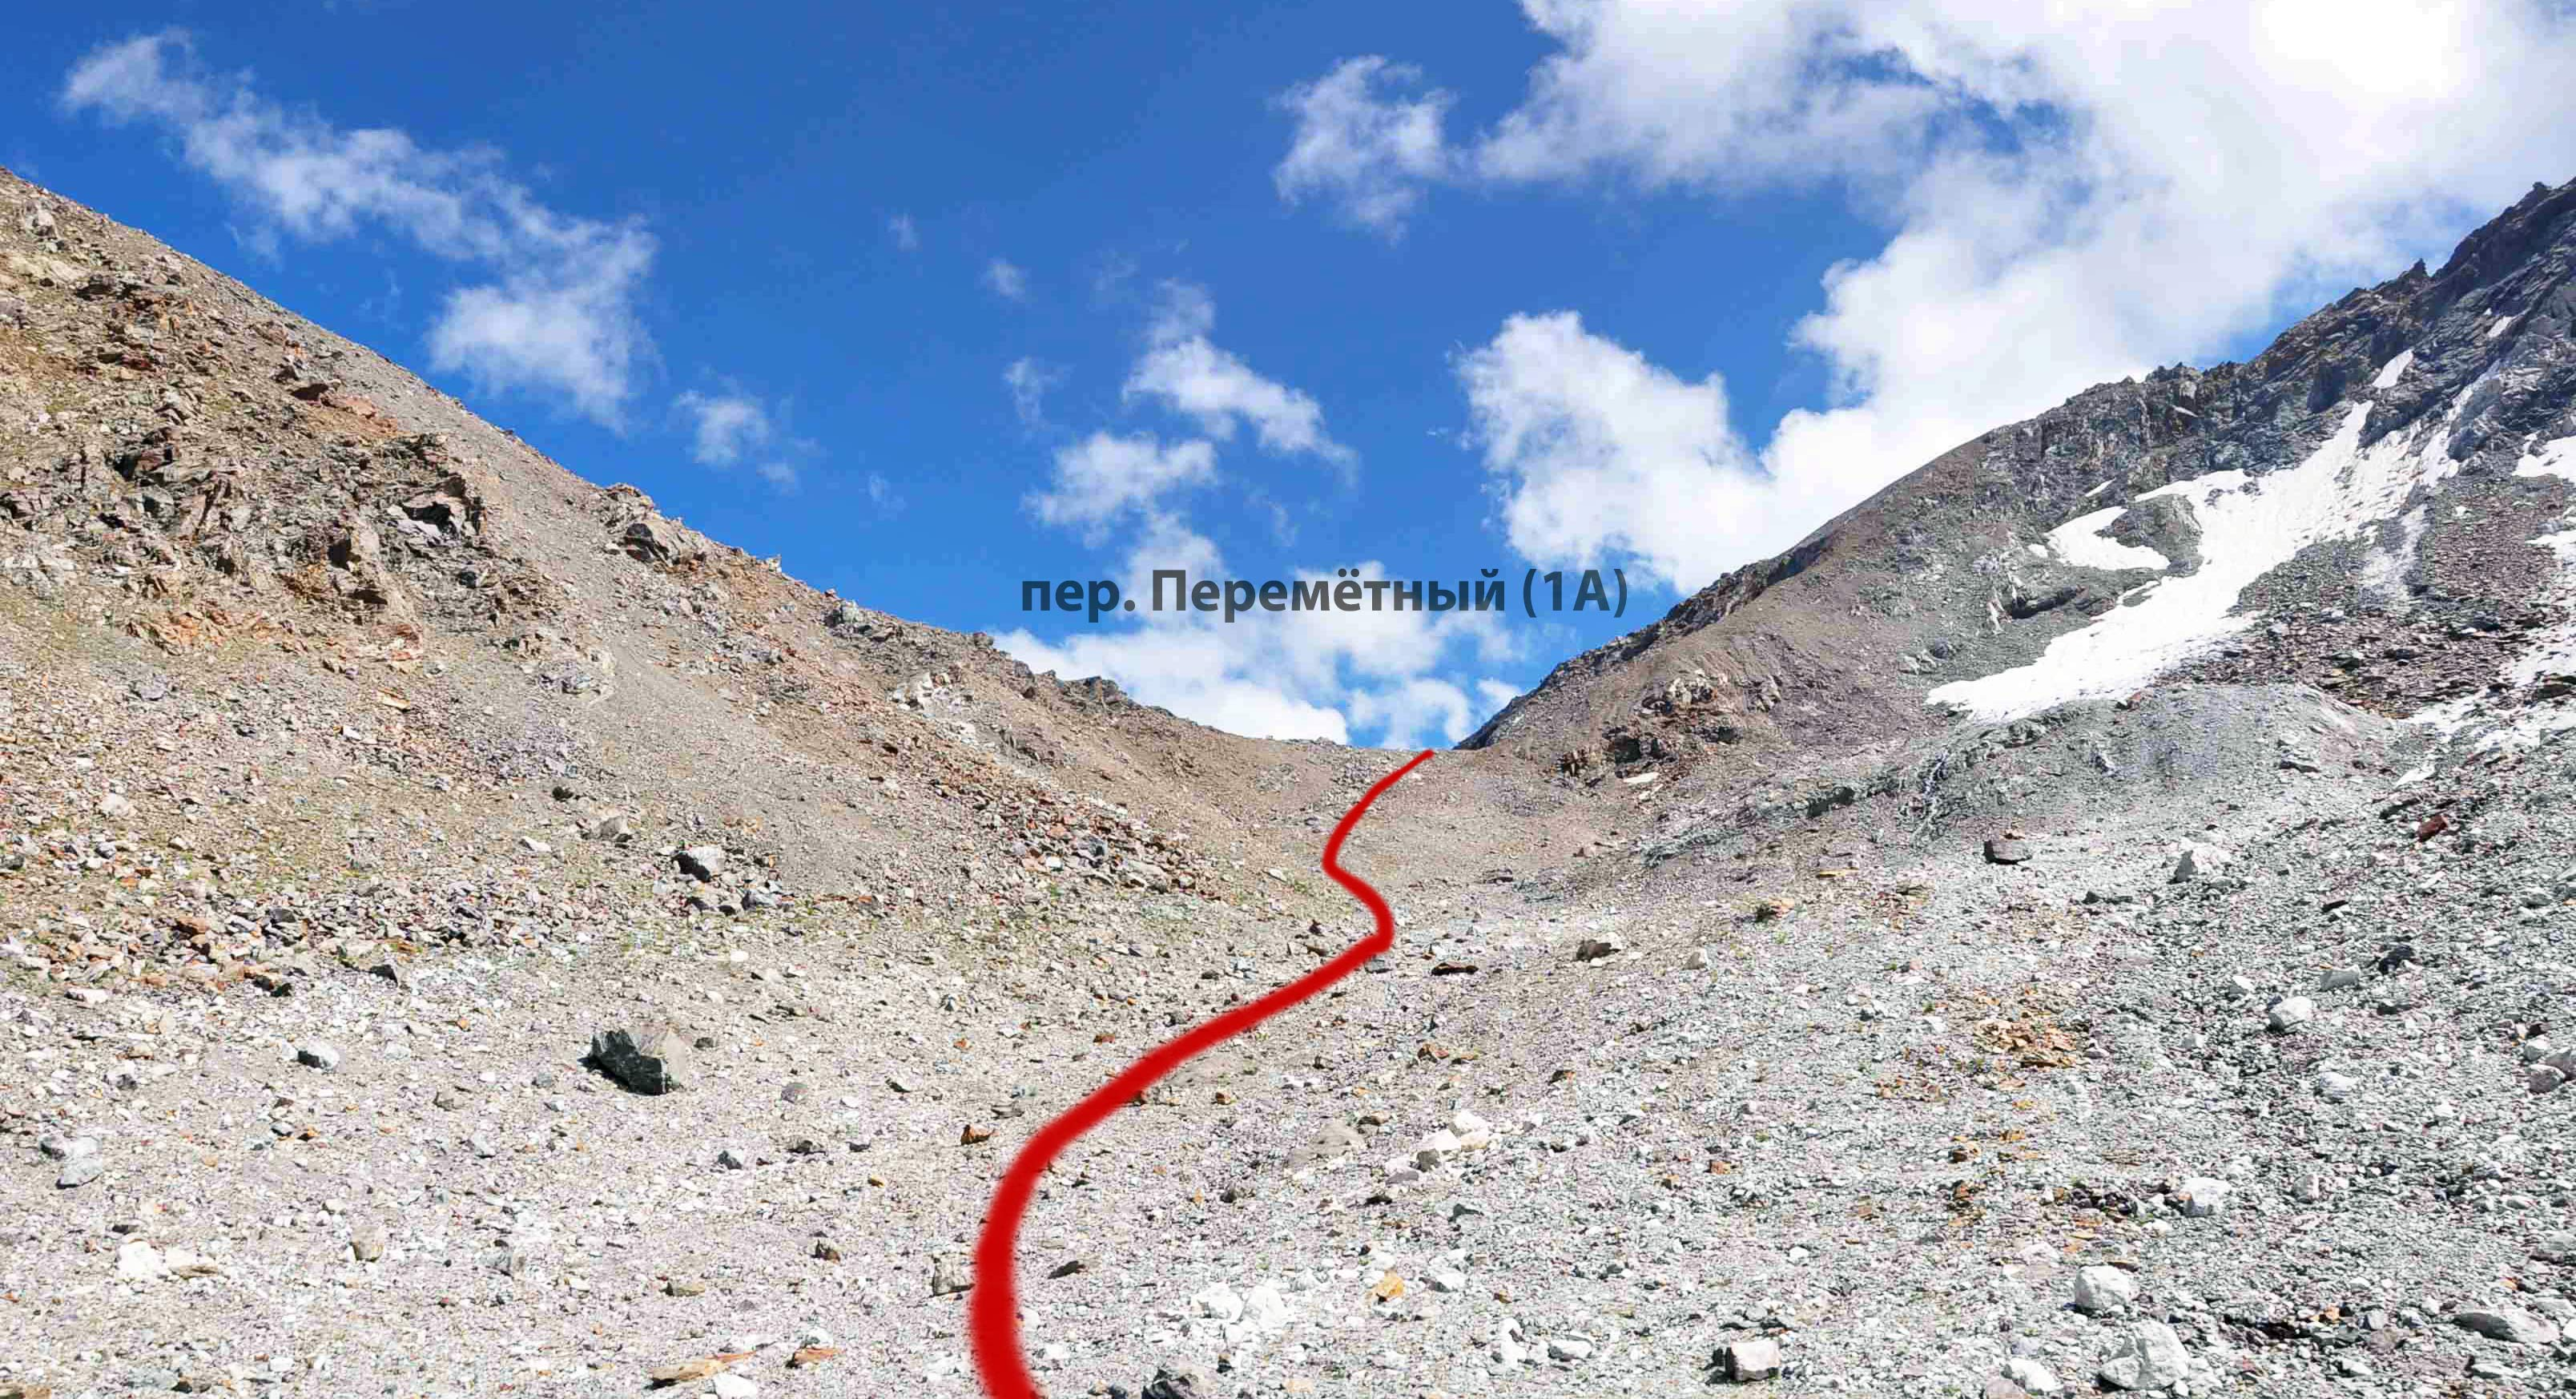
\includegraphics[width=0.7\linewidth]{../pics/DSC_0341.jpg}
	\caption{Перевальный взлёт}
	\label{fig:DSC_0341}
\end{figure} 

С задачей два справились в 14:33 (рис.~\ref{fig:DSC_0412}). На перевале сняли записку группы туристов из Ростова-на-Дону и Новочеркасска от 20.08.2019 (рис.~\ref{pic:peremetnyy}). Примечательно, что эта группа в своё время сняла записку Горной секции МФТИ под руководством Королёва Андрея от 2018 года~--- в этот поход ходила руковод.

\begin{figure}[h!]
	\centering
	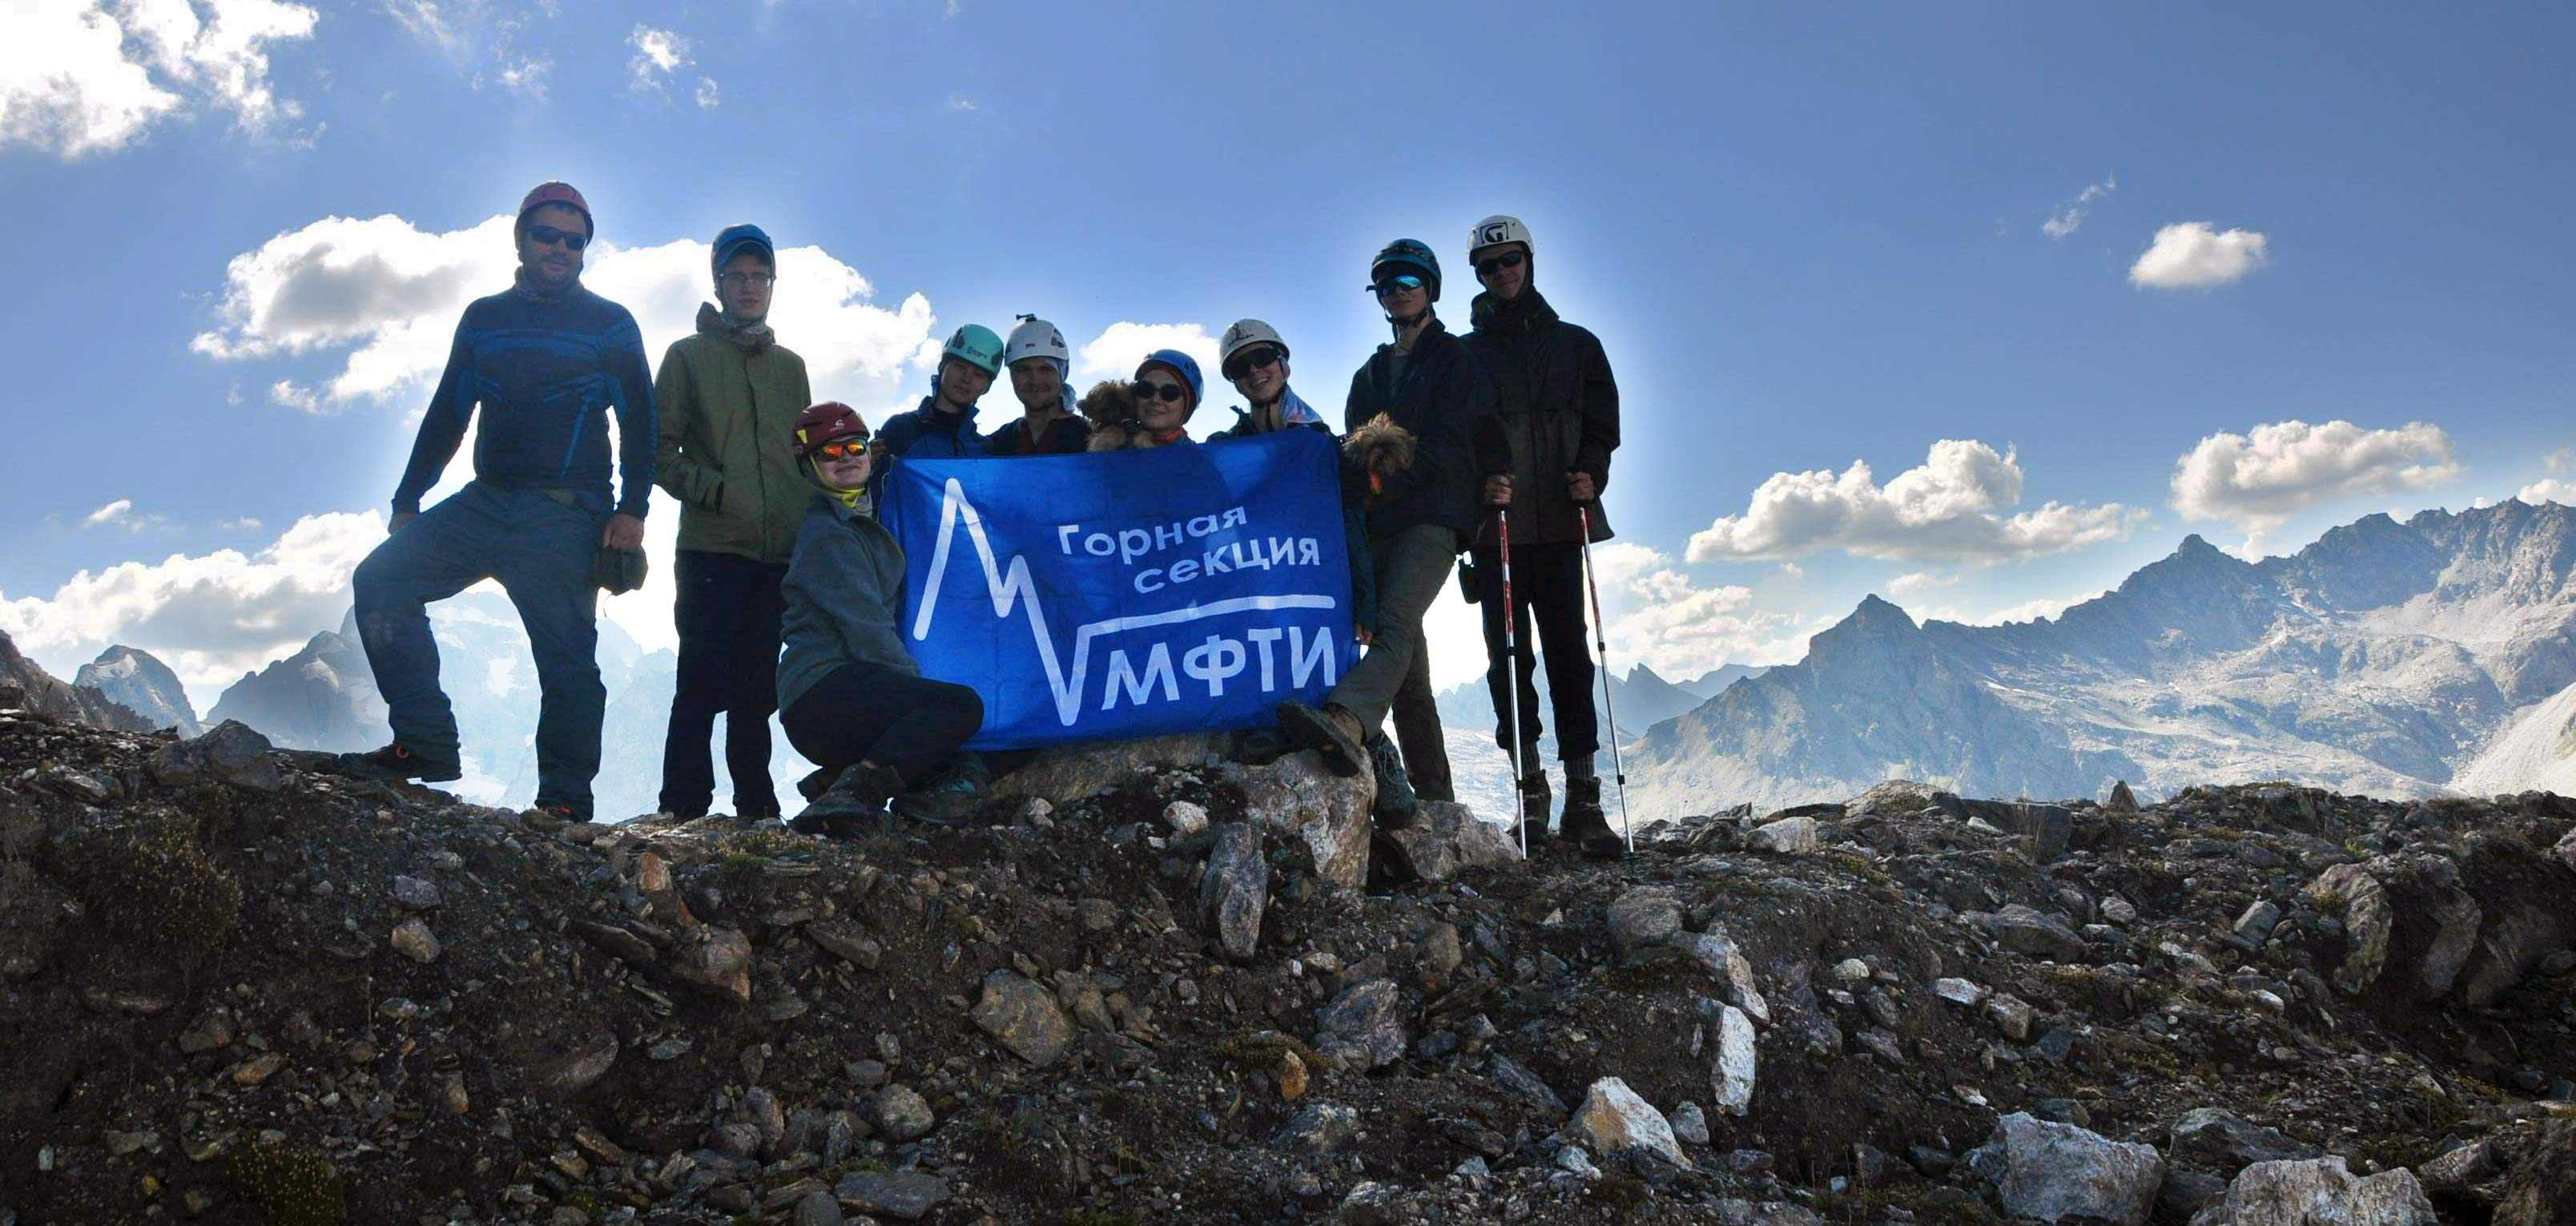
\includegraphics[width=0.7\linewidth]{../pics/DSC_0412 2.jpg}
	\caption{Группа на пер. Перемётный. Вид в д.р. Чунгур-Джар,}
	\label{fig:DSC_0412}
\end{figure} 


\begin{figure}[h!]
	\centering
	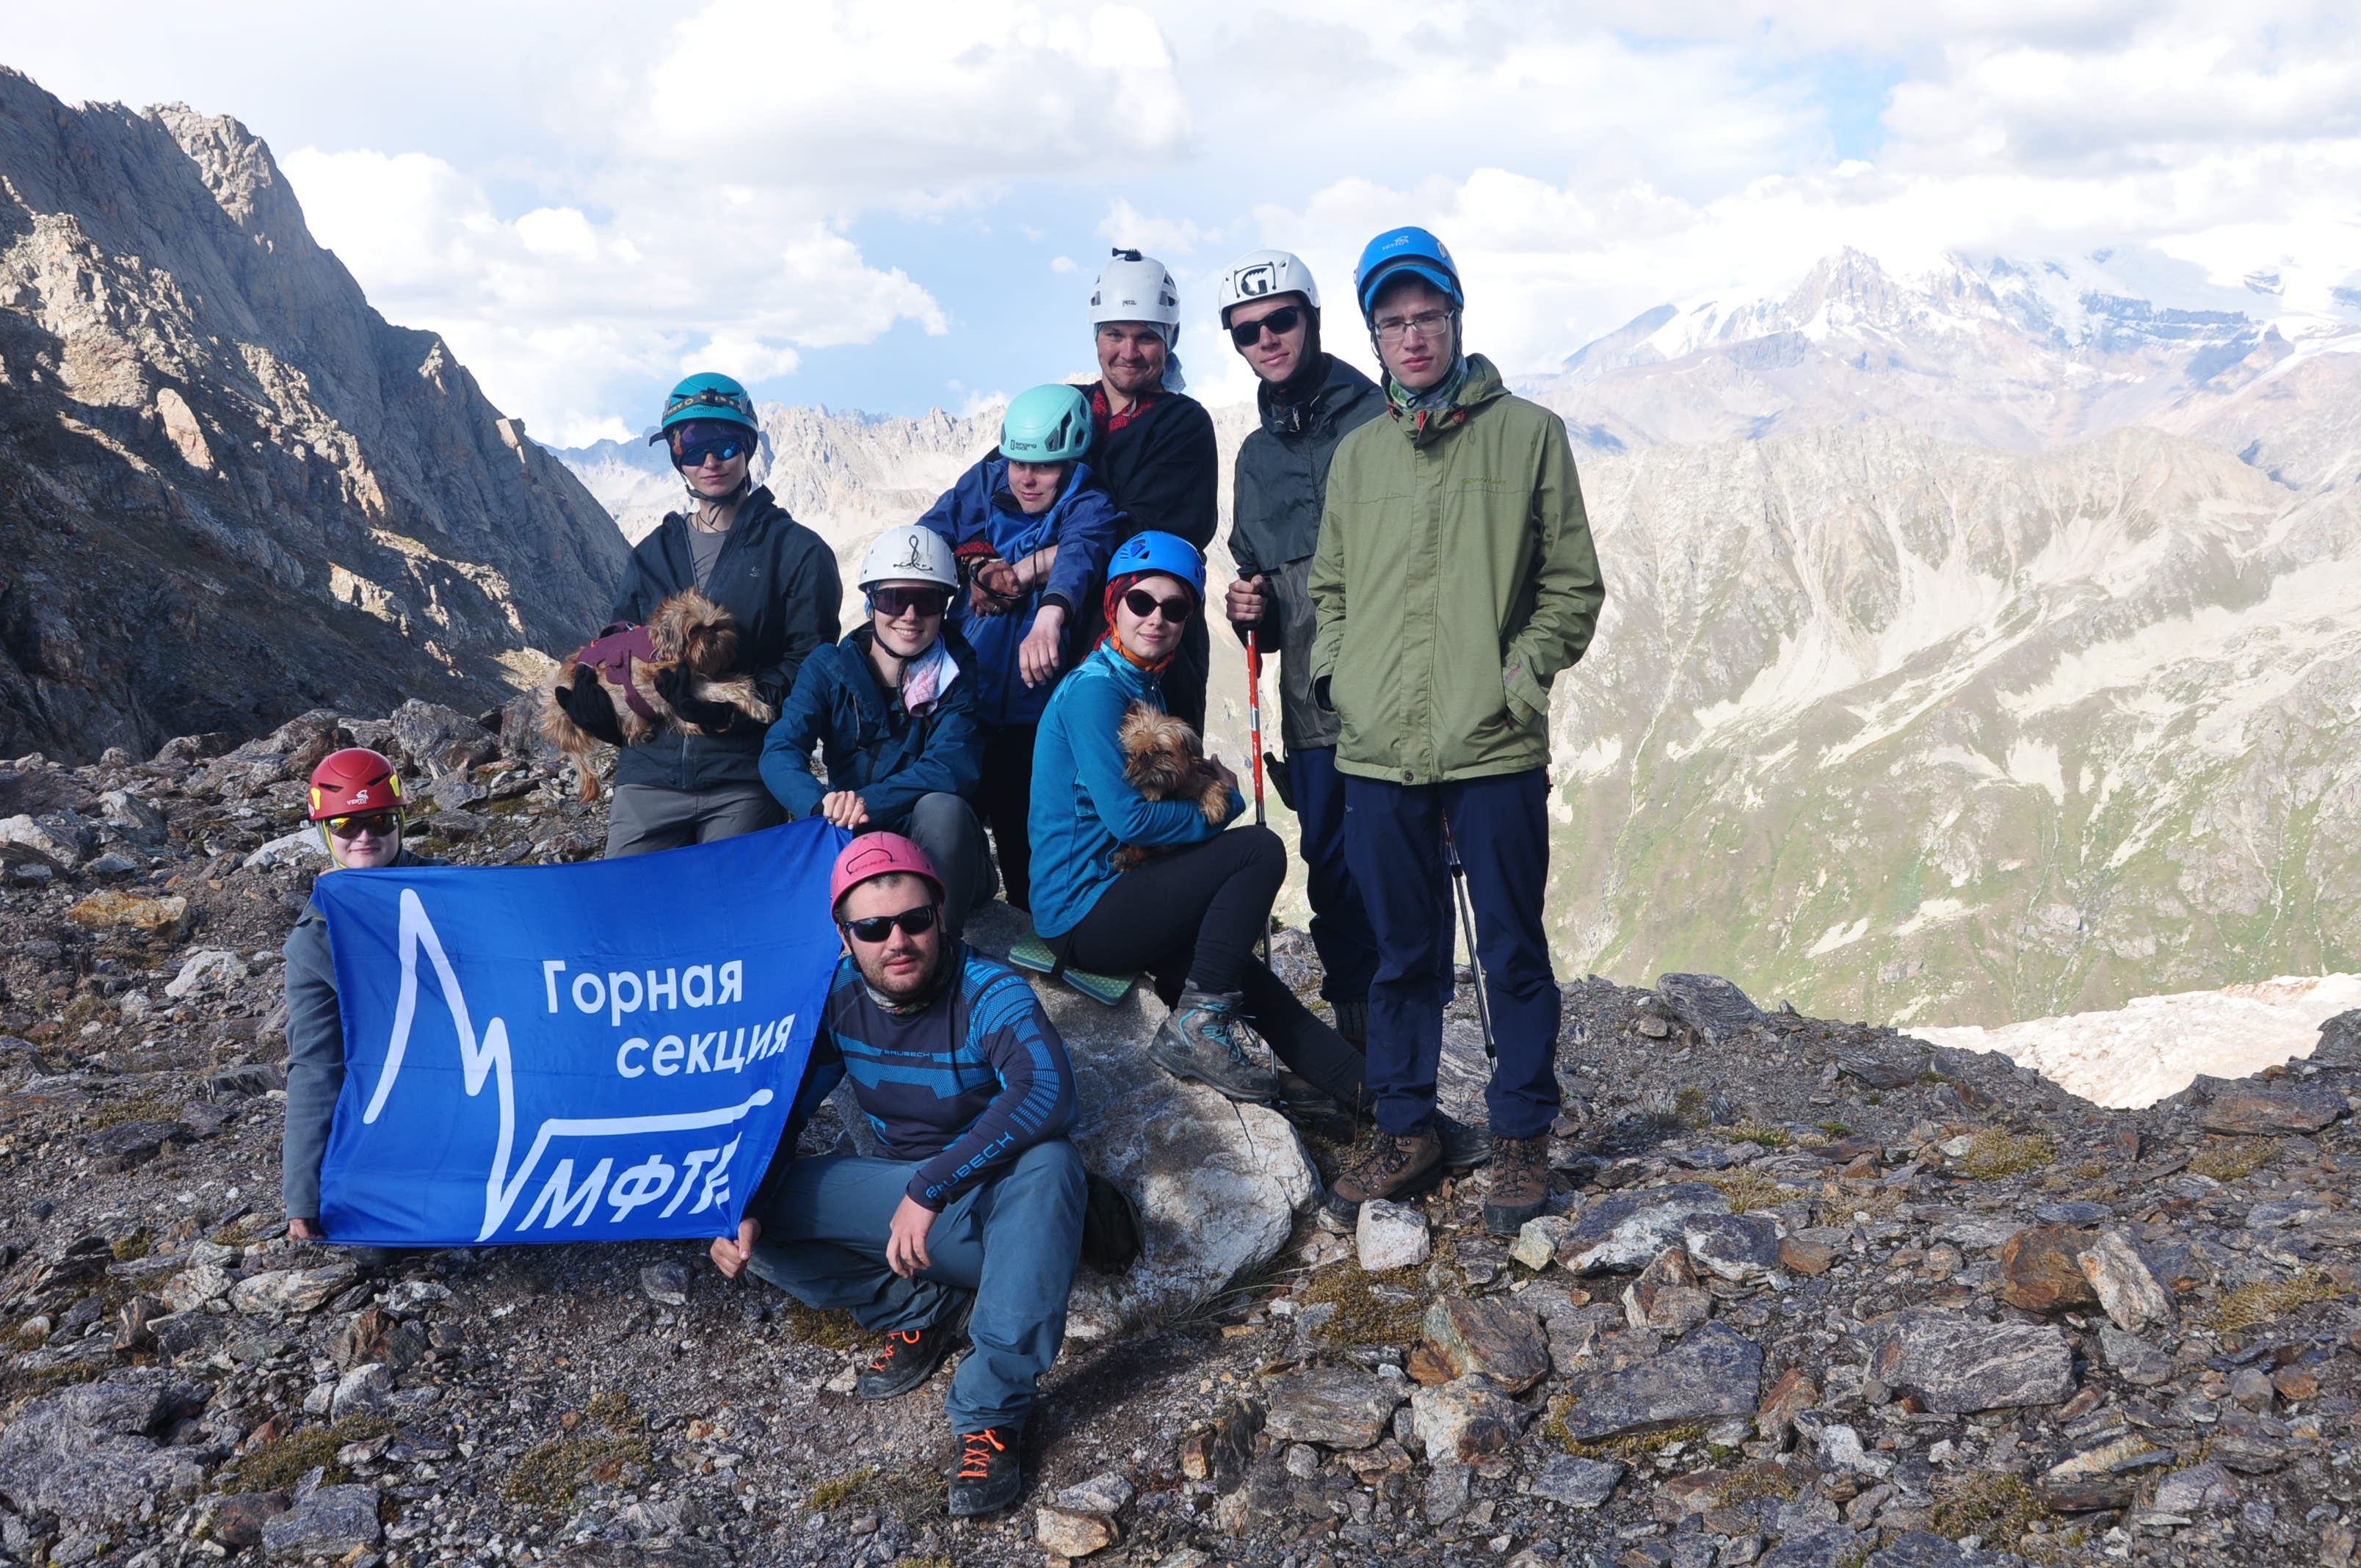
\includegraphics[width=0.7\linewidth]{../pics/DSC_0419 2.jpg}
	\caption{Группа на пер. Перемётный. Вид в д.р. Танышхан}
	\label{fig:DSC_0419}
\end{figure} 


\begin{figure}[h!]
	\centering
	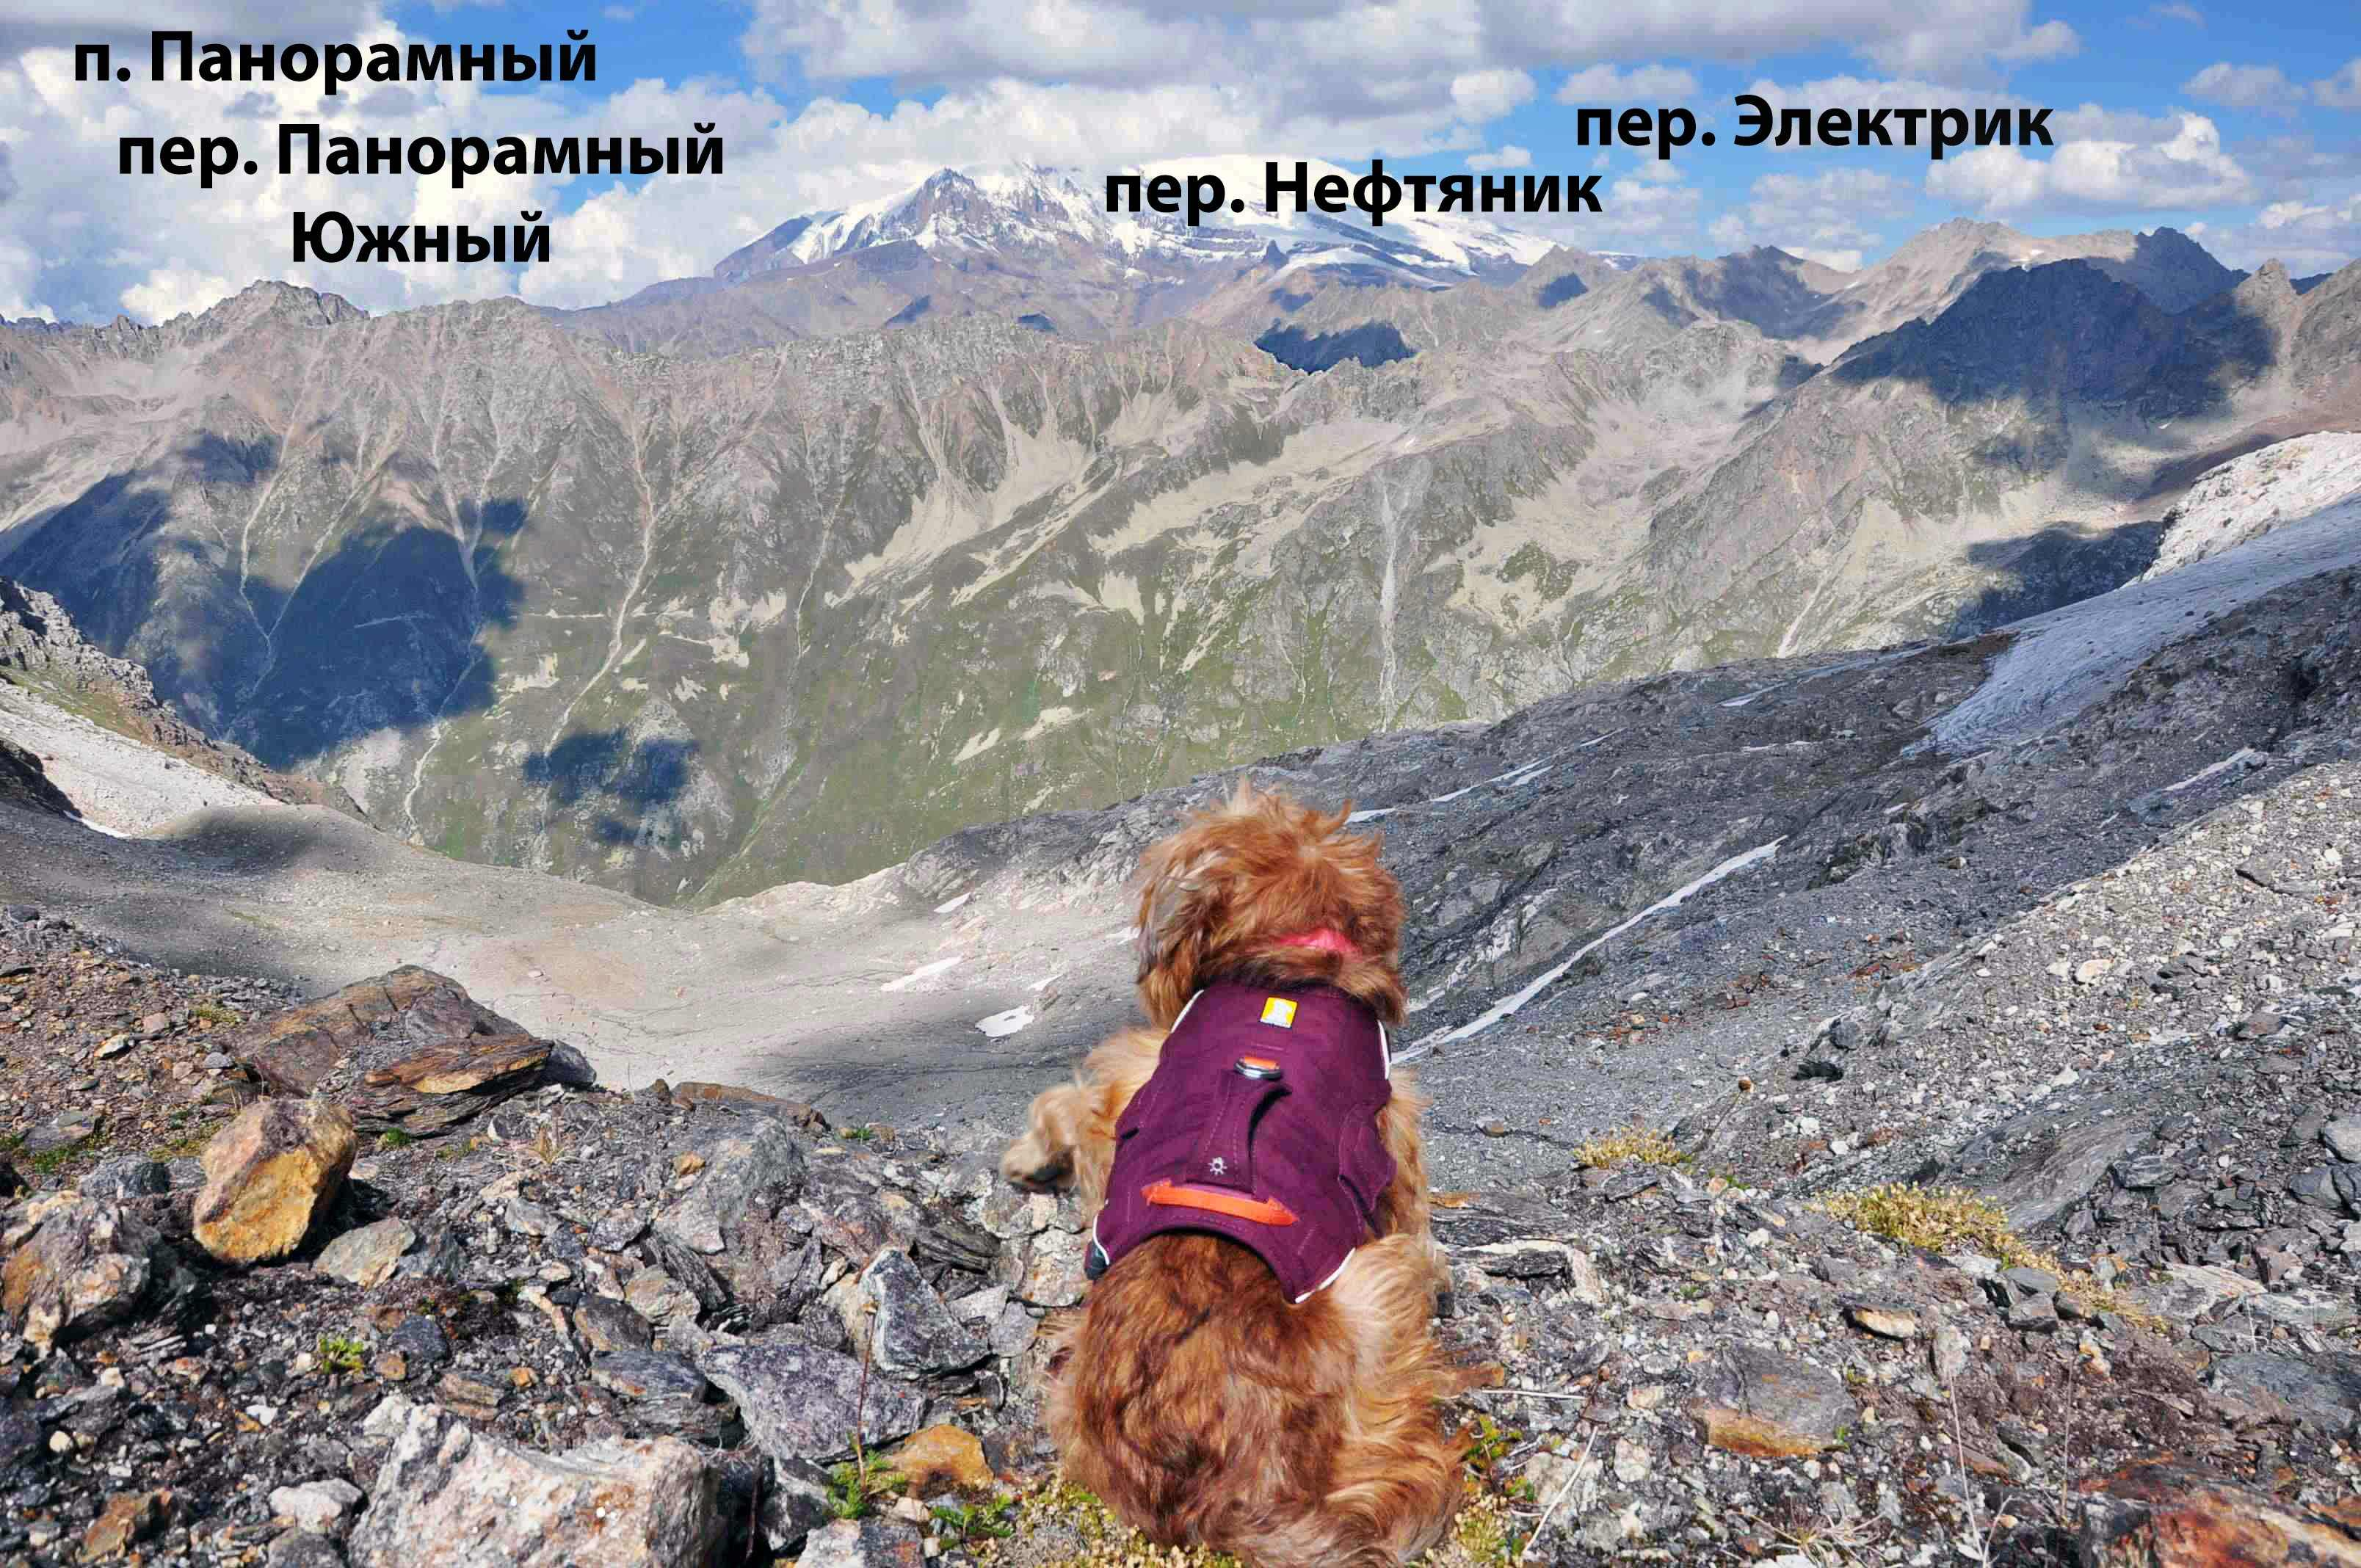
\includegraphics[width=0.7\linewidth]{../pics/DSC_0385 2.jpg}
	\caption{Вид с перевала в д.р. Танышхан}
	\label{fig:DSC_0385 2}
\end{figure} 

\textbf{Задачей номер три было} спуститься в низ, в д.р. Танышхан. 

\begin{figure}[h!]
	\centering
	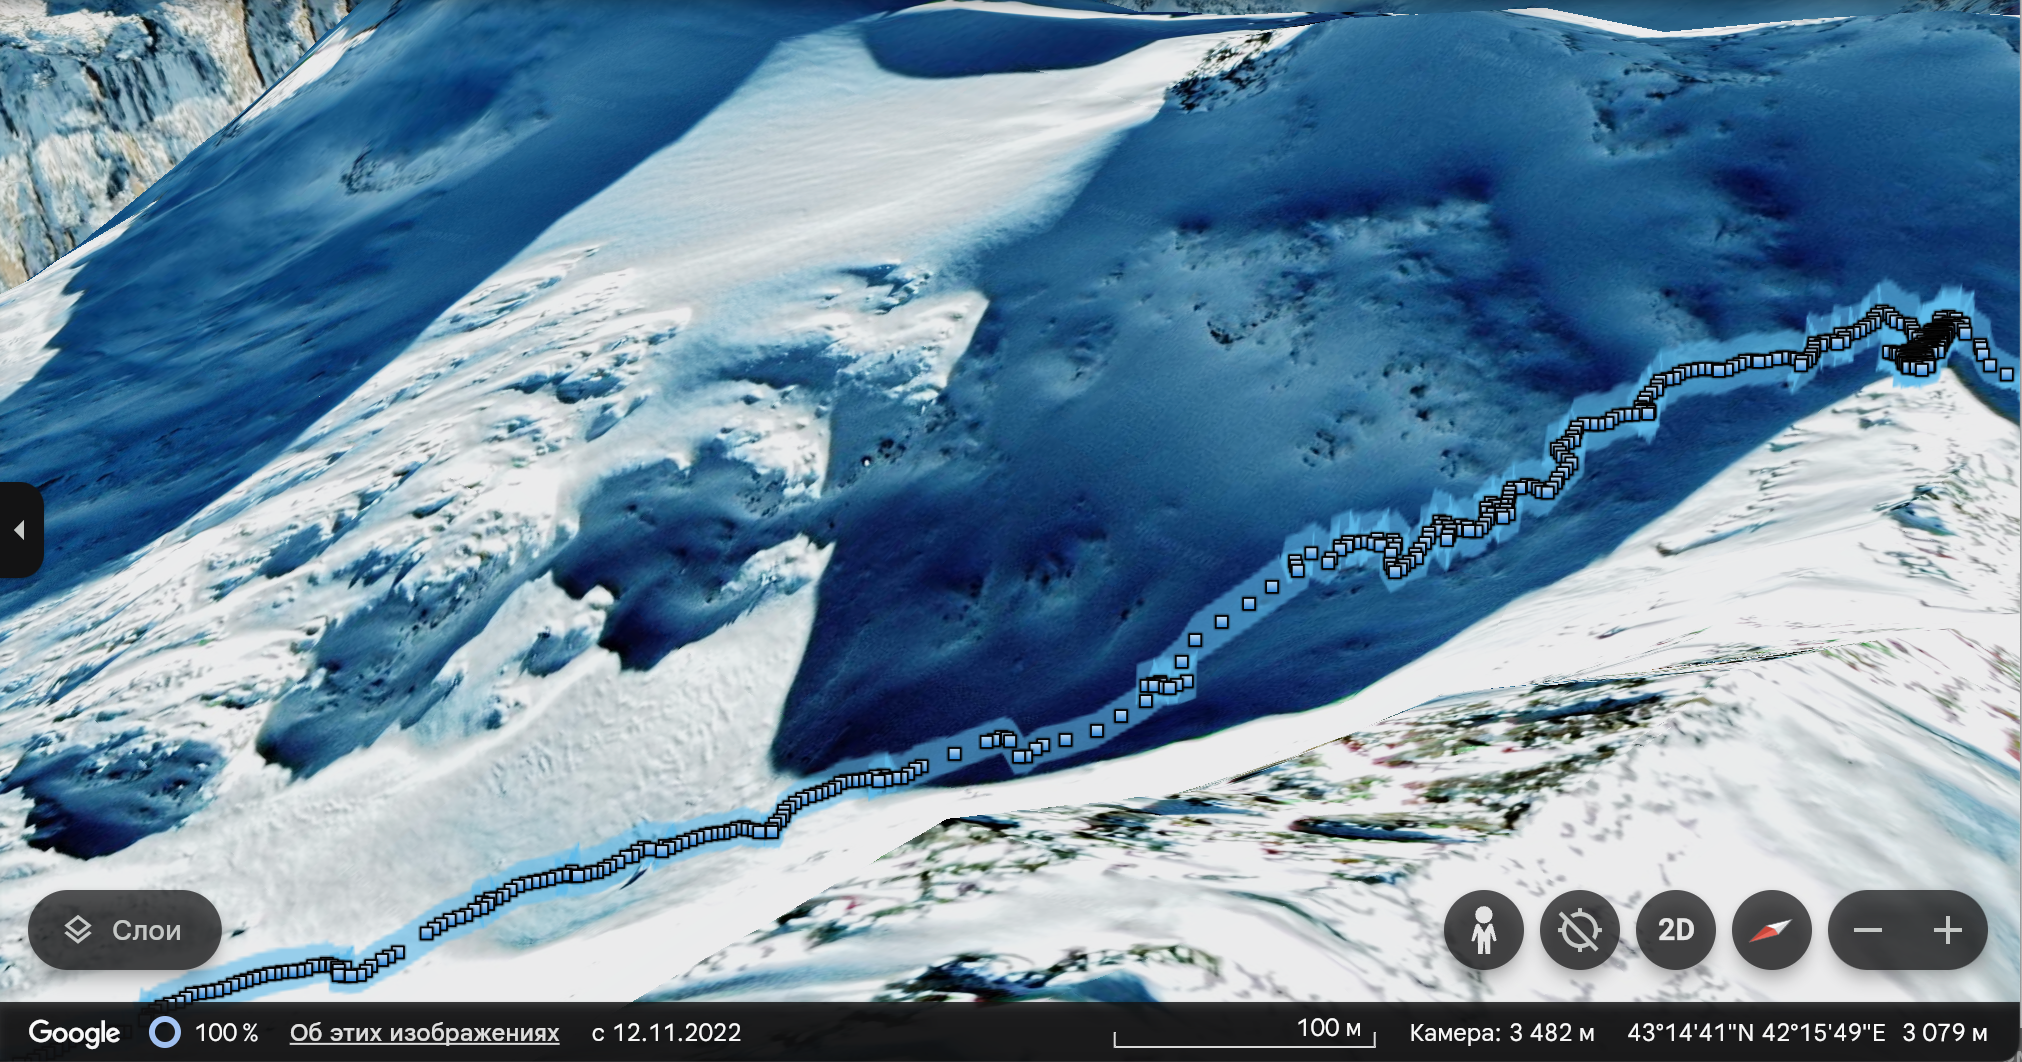
\includegraphics[width=0.7\linewidth]{../pics/google_earth/Peremetny-1.png}
	\caption{Спуск с перевала Перемётный на Google Earth: путь от седловины до выхода на ступень}
	\label{Peremetny-1}
\end{figure} 
\begin{figure}[h!]
	\centering
	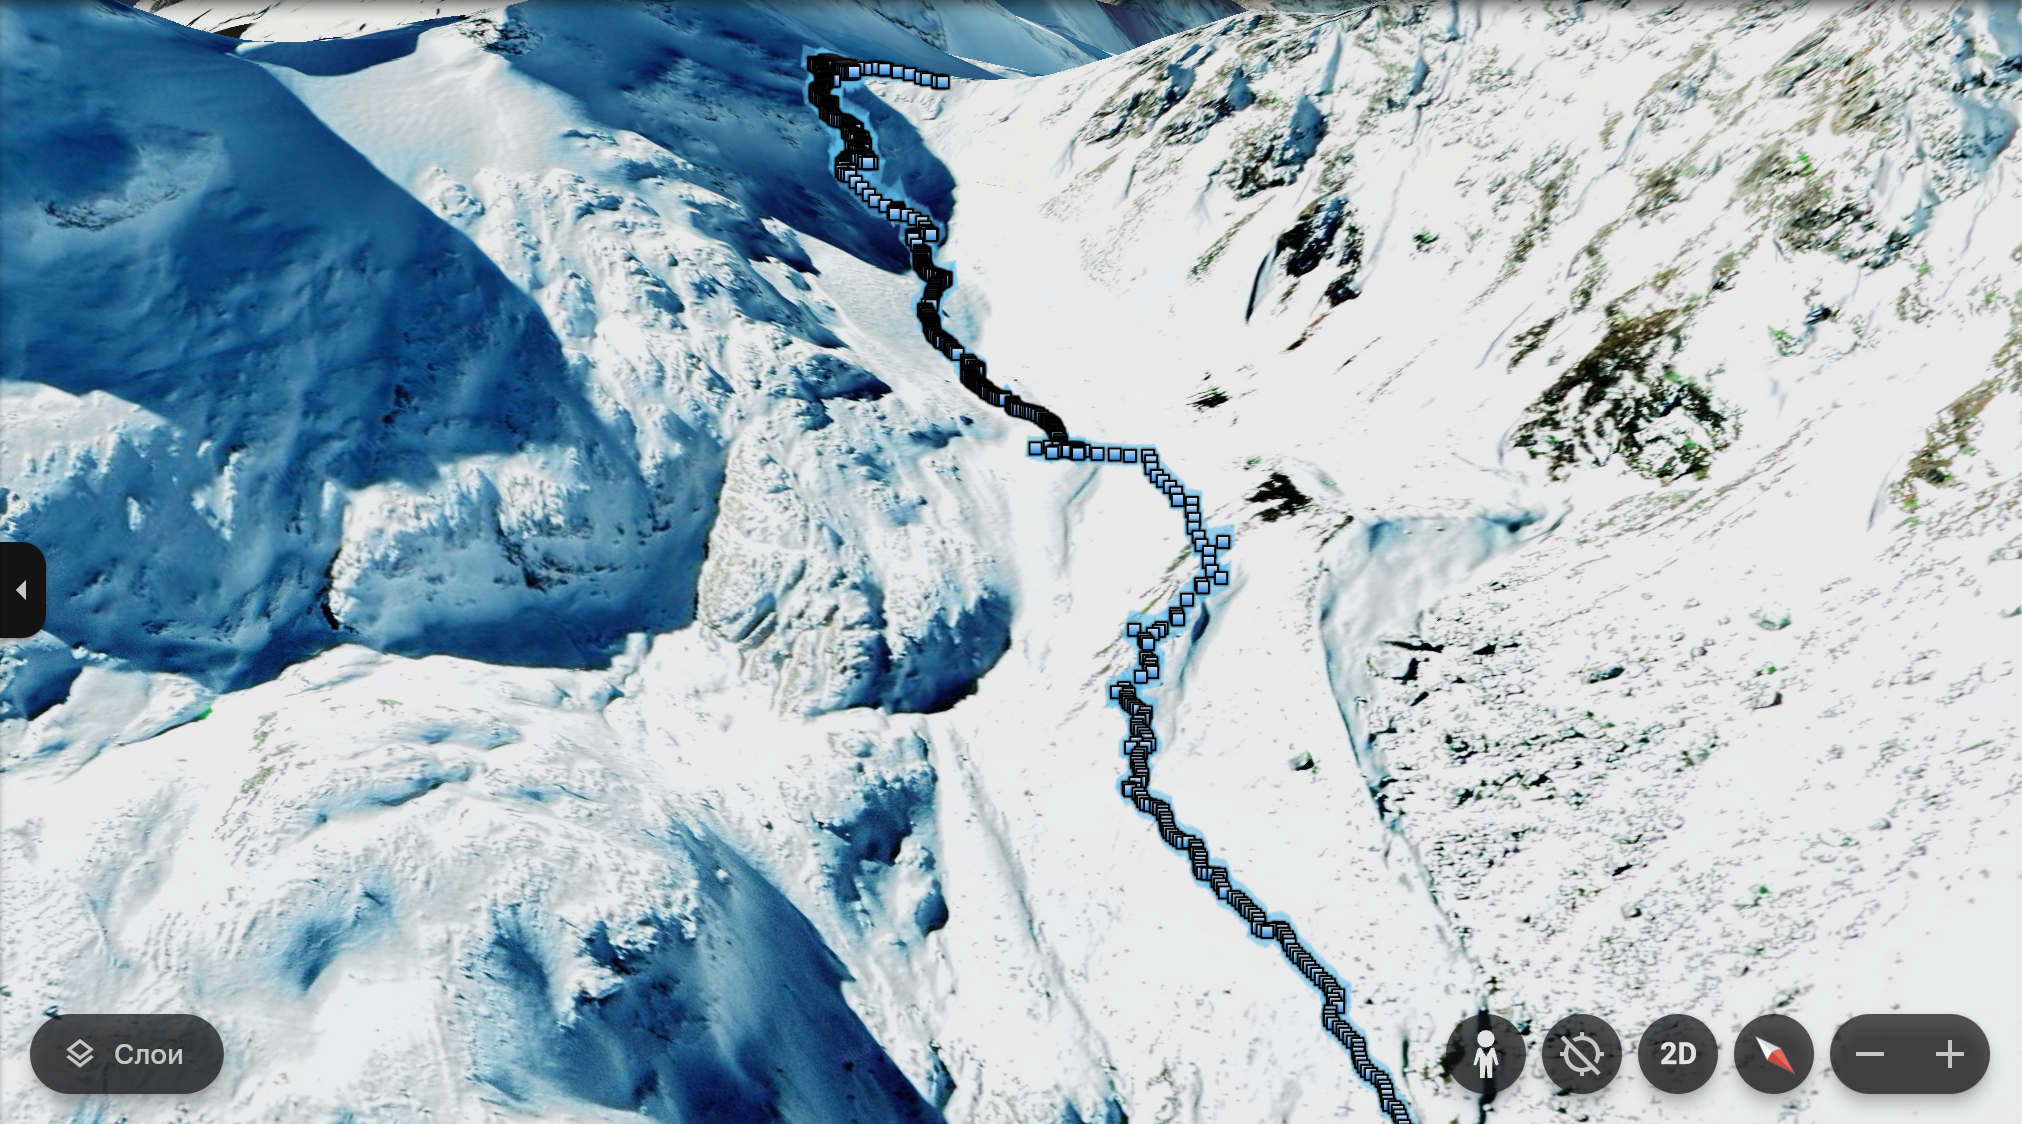
\includegraphics[width=0.7\linewidth]{../pics/google_earth/Peremetny-3.png}
	\caption{Спуск с перевала Перемётный на Google Earth: обход истока ручья с правого на левый берег и путь по гребню моренного вала}
	\label{Peremetny-3}
\end{figure} 
\begin{figure}[h!]
	\centering
	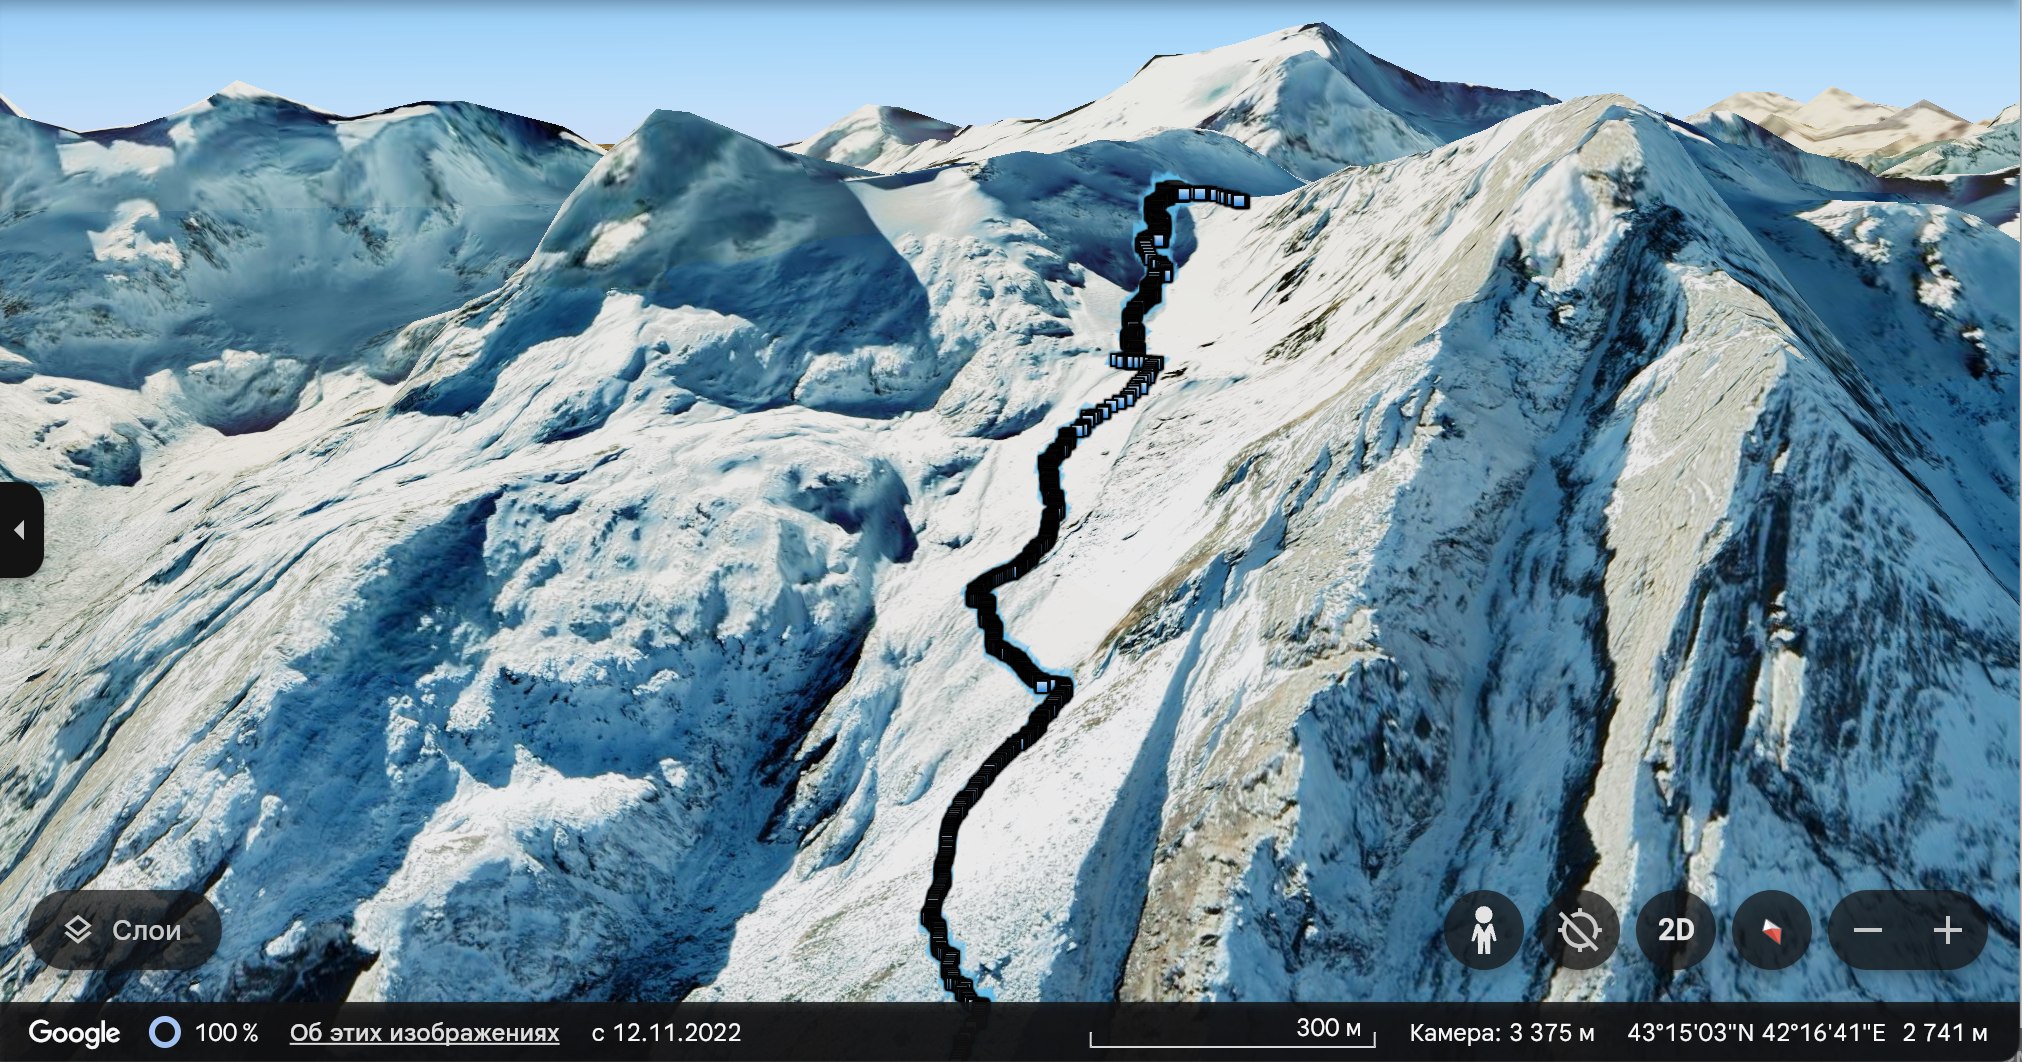
\includegraphics[width=0.7\linewidth]{../pics/google_earth/Peremetny-2.png}
	\caption{Спуск с перевала Перемётный на Google Earth: в нижней части скриншота --- спуск по травяному склону и выход на курумник}
	\label{Peremetny-2}
\end{figure} 


\begin{figure}[h!]
	\centering
	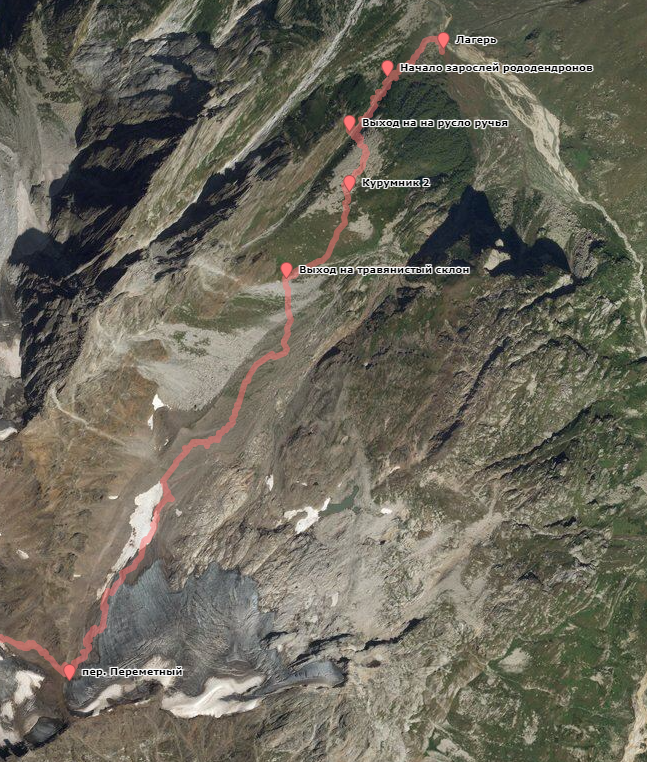
\includegraphics[width=0.7\linewidth]{../pics/perem_down.png}
	\caption{Спуск с перевала Перемётный}
	\label{perem_down}
\end{figure} 

Выдвинулись в 15:38. Вниз сначала шли по сыпухе забирая влево, усердно считая моренные валы, чтобы не ошибиться и не угодить в березняк. По пути старались расставлять турики, но время подгоняло, в маршруте мы были не уверены и на полпути это дело забросили. Потом начался травянистый склон, альпеншток альпеншточил на все 100. После спуска на 130 м выбрались на курумник, на котором не обошлось без лёгкого кровопролития. К сумеркам снова вышли на травянистый склон. Русло пересохшего ручья (N 43.25779\degree E 42.27107\degree), засыпанного крупными камнями, предоставило вариант спуска. К моменту, когда мы добрались до зарослей рододендронов, уже порядком стемнело (19:05), дальше по лощине шли с фонарикам. 

В 20:29 вышли на отличную стоянку на берегу реки Танышхан (N43.260205\degree,~E42.274914\degree). Поужинали и легли спать. С задачей три справились! 

\subparagraph{Описание от руководителя:} 
Спуск с перевала начали в 15:38. Согласно отчёту Анучиной \cite{Anuchina2019}, встать на стоянку можно было либо где-то в районе истока ручья, спустившись на 300 м ниже, либо уже в д/р Танышхан, сбросив полностью 900 м. Предполагалось, что практически наверняка реализуется первый, 300-метровый вариант. 

Первые 70 м спуска представляли из себя крутой осыпной склон, с живой осыпью среднего и крупного размера. Спускались по правому <<углу>> перевала, образованного собственно отрогом ГКХ Караганкая и отходящим от него гребнем. Шли плотной группой, зигзагом, с подстраховкой альпенштоком.  

Следующим этапом вышли на гребень моренного вала. Качество рельефа непосредственно на гребне не удовлетворило, поэтому моренный вал траверсировали по его правому борту, по серой вязкой осыпи, избегая полностью спускаться вниз --- чтобы не угодить под кромку снежника, который лежал с правой стороны от вала. Время движения~--- 30 мин ЧХВ от подножия крутого участка перевального взлёта.

После спуска с моренного вала шёл отличный пологий участок с постоянным уклоном и комфортным в плане перемещения рельефом, вплоть до выхода к истоку безымянного ручья~---левого притока р. Танышхан~--- и далее к краю ступени. Эта ступень может рассматриваться как ближайшее к перевалу пригодное место для стоянки, но Светлана Анучина стояла ниже. Продолжая сбрасывать высоту до уровня анучинской стоянки, мы пошли левым берегом ручья, по гребню моренного вала. 

На высоте стоянки были в 17:10. Неверно оценив, что за два оставшихся световых часа мы успеем спуститься на дно долины, решили продолжить движение. Двигались влево, огибая траверсом первый <<зелёный бугор>>: участок склона, который с этого ракурса перекрывает вид на дальнейший маршрут спуска. Этот участок прошли в 17:25. 

Далее в течение 1 часа ЧХВ двигались по травянистому склону. Скорость передвижения была ниже желаемой: сказывалась усталость и неопытность группы в передвижении по затяжным травянистым склонам. В 18:22 подошли под большой участок курумника, за которым располагалась лощина~--- финальный спуск на дно долины.

Последний курумник (рис.~\ref{fig:peremkurum}) оказался весьма протяжённым и шёл по-над всем участком криволесья. Уже смеркалось, и наиважнейшей задачей виделось дойти как можно скорее до конца курумника и спуститься в лощину. 

\begin{figure}[h!]
	\centering
	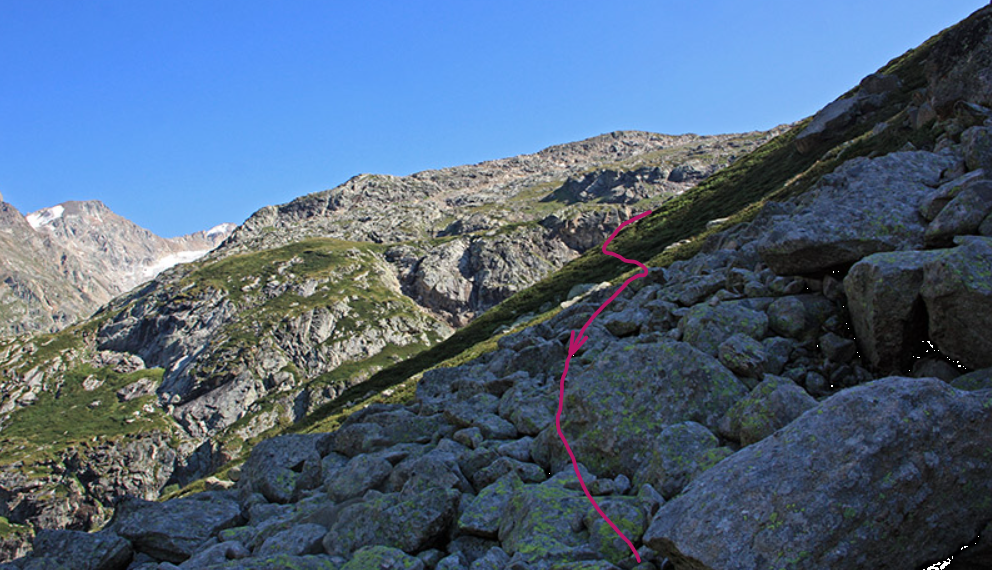
\includegraphics[width=0.7\linewidth]{../pics/peremkurum.png}
	\caption{Движение по курумнику. Фото Анучиной Светланы Красная линия~--- наш трек}
	\label{fig:peremkurum}
\end{figure} 

Точка выхода с курумника, которую группе удалось нащупать, оказалась, по-видимому, оптимальной: в этом месте, на участке склона от курумника до дна лощины, идут заросли рододенронов, в которых угадывается тропа. Ниже по склону начинаются скальные выходы, а выше лощина ещё более круто забирает вверх. 

Тем не менее, даже в нижней своей половине лощина была неожиданно крутой, и её дно было завалено камнями, которые на поверку оказывались живыми. Вдобавок, выпавшая роса ещё больше затрудняла движение. Этот участок при спуске с Перемётного, определённо, вызвал больше всего трудностей у группы. Начали движение вниз по лощине в 19:20, в темноте и с фонариками.

Наилучшей альтернативой спуску непосредственно по дну лощины, по камням, мог бы быть спуск зигзагами (<<галсами>>) по склону левее, но в данном случае сильно сказалось то, что участники недостаточно хорошо владели техникой подстраховки альпенштоком, поэтому последние 300 м спуска по вертикали заняли 45 мин. ЧХВ. 

К широким разливам р. Танышхан, <<Танышханскому аэродрому>>, спустились в 20:29. Координаты м.н. N43.260205\degree,~E42.274914\degree. Здесь активно пасутся коровы; воду для приготовления пищи брали не в Танышхане, а в одном из его левых притоков, стекающих со склона. Он находился в 50 м вверх по течению от лагеря.
В лагере участники Дима Сингалевич и Маша Семено сообщили о своём решении сойти с маршрута в Хурзуке. Дима --- формально из за проблем с коленями, но, как выяснили позже, из-за того, что решения руководителя превысили допустимый лично для него уровень риска. Маша --- из-за того что, волонтёря накануне на ужине, промокла и в итоге простыла. Также, возможно, её сильно измотало психологически хождение ночью.

\begin{table}[h!]
	\centering
	\begin{tabular}{|c|c|c|c|c|c|} 
		\hline 
		Этап & ЧХВ \\ 	
		\hline 
		Подъём от места ночевки до языка ледника  & 02:41 \\
		Подъём от языка ледника до седловины  & 00:40 \\
		Спуск с седловины перевала Переметный до лощины & 02:41\\ 
		Спуск по лощине до д.р. Чиринкол & 01:23\\ 
		Спуск с места ночёвки до слияния рек Чиринкол и Кубань & 04:10 \\
		
		\hline
		\textsc{Полное время подъёма на перевал  }& 03:21\\
		\textsc{Полное время спуска с перевала }& 08:14 \\
		\textsc{Полное время прохождения перевала }& 11:35 \\
		\hline
	\end{tabular}
	\caption{Расклад времени, пер. Перемётный}
\end{table}

\paragraph{Выводы и рекомендации:} Пер. Перемётный остаётся малохоженным по сравнению с другими перевалами Гвандры и, по нашему мнению, незаслуженно. Отличается разнообразием форм рельефа, выразительным горным хребтом, красивыми видами на окрестности. Несмотря на то, что тропы на подъём и спуск нет, технически перевал не является сложным и полностью соответствует своей категории. Однако, основываясь на нашем опыте и опыте предыдущих групп, рекомендуем закладывать непосредственно на его прохождение не один, а два дня. Впрочем, если физические возможности группы превышают средние, то пройти спуск с Перемётного можно и за один день, уложившись до наступления темноты.

\clearpage